% ======================================================
%         1. GIỚI THIỆU (INTRODUCTION)
% ======================================================
% \section{}: tiêu đề cấp 1, tự động đánh số
% Mục này giới thiệu bối cảnh và lý do chọn đề tài
\section{Giới thiệu}

Trong bối cảnh sự kiện thể thao quốc tế quy mô lớn như World Cup 2026 và ASIAD 2026 sắp diễn ra, nhu cầu xem thể thao trực tuyến tại Việt Nam đang gia tăng mạnh mẽ. Nhiều nền tảng OTT (Over-The-Top) đã và đang phát triển để đáp ứng nhu cầu này, trong đó VTVPrime và FPTPlay là hai dịch vụ phổ biến nhất hiện nay. Báo cáo này tập trung phân tích hai nền tảng này từ góc độ HCI (Human-Computer Interaction) nhằm đánh giá trải nghiệm người dùng, xác định các vấn đề thiết kế hiện có, và đề xuất hướng cải thiện dựa trên các nguyên tắc HCI cơ bản.

\subsection{Lý do chọn sản phẩm}

\textbf{VTVPrime} là nền tảng streaming OTT của Tổng Công ty Truyền hình Cáp Việt Nam (VTVcab), doanh nghiệp trực thuộc Đài Truyền hình Việt Nam (VTV). Được thành lập từ năm 1995 với tên gọi ban đầu là VCTV, VTVcab đã phát triển mạnh mẽ từ hệ thống truyền hình cáp truyền thống sang các nền tảng số hiện đại. VTVprime là nền tảng OTT đầu tiên và duy nhất tại Việt Nam có giấy phép mạng xã hội (tính đến năm 2025), cho phép người dùng không chỉ xem nội dung mà còn tương tác qua việc tạo tài khoản, bình luận, thảo luận cộng đồng, thả cảm xúc và xếp hạng chương trình. Với vị thế là nhà cung cấp nội dung chính thống, VTVprime là một trong các nền tảng phát sóng chính của hệ sinh thái VTV, bao gồm cả các sự kiện thể thao lớn mà VTV sở hữu bản quyền như World Cup 2026, ASIAD, UEFA Euro, Premier League và các giải đấu bóng đá trong nước.

\textbf{FPTPlay} là thương hiệu truyền hình và nội dung số thuộc sở hữu của Công ty Cổ phần Viễn thông FPT (FPT Telecom), trực thuộc Tập đoàn FPT. Phát hành lần đầu vào ngày 11 tháng 9 năm 2013, FPT Play đã phát triển thành một trong những dịch vụ OTT hàng đầu tại Việt Nam. Theo báo cáo của Group M, FPT Play chiếm thị phần lớn nhất trên thị trường OTT tại Việt Nam với 39\% thị phần, đứng thứ 2 trong top các ứng dụng được xem nhiều nhất trên TV thông minh chỉ sau YouTube. Hiện tại, FPT Play có hơn 36 triệu lượt tải về và 25 triệu người dùng, cung cấp gần 200 kênh truyền hình trong và ngoài nước cùng kho nội dung đa dạng từ phim truyện, chương trình truyền hình, tin tức, thiếu nhi đến thể thao và gameshow. FPT Play cũng sở hữu bản quyền Vòng loại thứ 3 World Cup – Khu vực châu Á, các giải đấu cấp CLB thuộc UEFA từ 2021-2024 và giải bóng đá Ngoại Hạng Anh từ nửa mùa giải 2025/2026 đến năm 2031.

Việc lựa chọn hai nền tảng này dựa trên sự phổ biến và vị thế của chúng trên thị trường streaming thể thao tại Việt Nam. Cả hai nền tảng đều sở hữu bản quyền các sự kiện thể thao lớn và có lượng người dùng đáng kể. Điều này tạo điều kiện thuận lợi cho việc phân tích HCI vì:

\begin{itemize}
  \item Sở hữu bản quyền sự kiện thể thao lớn giúp thu hút đa dạng phân khúc người dùng, cho phép phân tích HCI trên nhiều loại người dùng khác nhau.
  \item Sản phẩm phổ biến thường có nhiều phản hồi công khai về trải nghiệm người dùng qua các kênh đánh giá, diễn đàn và mạng xã hội, giúp thu thập thông tin về các vấn đề HCI thực tế.
\end{itemize}

Phân tích so sánh hai nền tảng phổ biến này sẽ giúp nhóm hiểu rõ hơn về các xu hướng thiết kế HCI trong streaming thể thao, từ đó rút ra các bài học về những phương pháp thiết kế hiệu quả và các vấn đề cần tránh. Phân tích này sẽ là cơ sở quan trọng cho việc đề xuất giải pháp thiết kế trong các giai đoạn tiếp theo của dự án.

% ======================================================
%          2. SẢN PHẨM 1: VTVPRIME
% ======================================================
% Mục này phân tích chi tiết sản phẩm VTVPrime
% \section{}: tiêu đề cấp 1 (sản phẩm)
% \subsection{}: tiêu đề cấp 2 (tên, domain, use case...)
\section{Sản phẩm 1: VTVPrime}

% --- 2.1 Tên sản phẩm & Domain ---
% Bảng thông tin tổng quan về VTVPrime
% tabularx với cột X: tự động giãn cột theo \textwidth
\subsection{Tên sản phẩm \& Domain}

% Bảng thông tin tổng quan sản phẩm
% |l|X|: cột trái cố định + cột phải co giãn tự động
\begin{center}
\begin{tabularx}{\textwidth}{|l|X|}
\hline
\textbf{Thông tin} & \textbf{Chi tiết} \\
\hline
\textbf{Tên sản phẩm} & VTVPrime \\
\hline
\textbf{Domain} & Nền tảng xem thể thao, phim và chương trình truyền hình trực tuyến \\
\hline
\textbf{Nền tảng} & Web (\url{https://vtvprime.vn}), Mobile (iOS/Android), TV thông minh \\
\hline
\textbf{Nhà phát hành} & Tổng Công ty Truyền hình Cáp Việt Nam (VTVcab), doanh nghiệp trực thuộc Đài Truyền hình Việt Nam (VTV) \\
\hline
\end{tabularx}          % Kết thúc bảng tabularx
\end{center}

% --- 2.2 Đối tượng người dùng ---
% Phân khúc hóa người dùng theo hành vi, bối cảnh và nhân khẩu học
% 5 phân khúc: A (cứng), B (sự kiện), C (cầu may), D (catch-up), E (phụ trợ)
\subsection{Đối tượng người dùng}

\subsubsection{Đặc điểm nhân khẩu học và hành vi theo độ tuổi}

Theo báo cáo Digital 2026 \ref{ref:datareportal}, Việt Nam hiện có khoảng 85,6 triệu người dùng Internet (chiếm 84,2\% dân số). Với độ tuổi trung bình là 33,4, tập khách hàng của các nền tảng OTT vô cùng đa dạng, dẫn đến những khác biệt rõ rệt về năng lực tiếp nhận công nghệ và kỳ vọng trải nghiệm.

\begin{center}
\begin{tikzpicture}
\begin{axis}[
    ybar,
    symbolic x coords={18-24, 25-34, 35-44, 45-54, 55-64, 65+},
    xtick=data,
    nodes near coords,
    nodes near coords align={vertical},
    ymin=0, ymax=20,
    ylabel={Tỷ lệ (\%)},
    xlabel={Độ tuổi},
    width=0.8\textwidth,
    height=6cm,
    bar width=15pt,
]
\addplot coordinates {(18-24,9.2) (25-34,14.4) (35-44,16.3) (45-54,12.7) (55-64,10.4) (65+,9.5)};
\end{axis}
\end{tikzpicture}
\end{center}

\medskip\noindent Qua phân tích số liệu thực tế, nhóm nghiên cứu xác định 4 nhóm đối tượng trọng tâm với các đặc thù về HCI như sau:

\begin{itemize}
    \item \textbf{Nhóm Gen Z (18--24 tuổi)}: Đây là thế hệ "bản địa số" (Digital Natives) – những người sinh ra và lớn lên trong kỷ nguyên Internet, coi công nghệ là một phần tất yếu của cuộc sống. Họ ưu tiên tốc độ và tính trực quan, có xu hướng thao tác nhanh và ít kiên nhẫn với các luồng giao diện rườm rà. Đối với nhóm này, phản hồi tức thì (immediate feedback) là yếu tố tiên quyết để duy trì lòng trung thành với ứng dụng.
    
    \item \textbf{Nhóm lao động trẻ (25--44 tuổi)}: Chiếm tỷ trọng lớn nhất (30,7\%), đây là nhóm người dùng có tính chọn lọc cao. Họ đề cao sự ổn định, tính thực dụng và các mô hình tương tác quen thuộc (design patterns) để tối ưu hóa thời gian sử dụng giữa lịch trình bận rộn. Họ không có xu hướng chạy theo các ứng dụng mới nhất nếu không thực sự cần thiết, mà ưu tiên những giải pháp đã được chứng minh hiệu quả và đáp ứng đủ nhu cầu hiện tại.
    
    \item \textbf{Nhóm trung niên (45--54 tuổi)}: Nhóm này tiếp cận công nghệ một cách thận trọng. Họ ưu tiên các giao diện có cấu trúc rõ ràng, nhất quán và cần những chỉ dẫn cụ thể khi có sự thay đổi về tính năng hoặc luồng xử lý.
    
    \item \textbf{Nhóm người lớn tuổi (55 tuổi trở lên)}: Khi tuổi tác tăng, thị lực và khả năng điều khiển thiết bị thường không còn linh hoạt như trước. Do đó, nhóm này dễ gặp khó khăn với các giao diện có chữ nhỏ, biểu tượng phức tạp hoặc thao tác đòi hỏi độ chính xác cao. Họ cần các thiết kế có tương phản rõ, nút bấm lớn, ngôn ngữ đơn giản và luồng thao tác ổn định, không thay đổi đột ngột. Đây là nhóm phản ánh rõ nhất các ràng buộc về năng lực con người trong thiết kế hệ thống.
\end{itemize}

\subsubsection{Phân khúc người dùng dựa trên mức độ gắn kết và hành vi xem}

Dựa trên các nghiên cứu chuyên sâu về thị trường streaming thể thao (Kantar, Disney Advertising, Parks Associates), nhóm nghiên cứu phân loại người dùng VTVPrime thành các phân khúc dựa trên động cơ và bối cảnh sử dụng:

\bigskip
\begin{center}
\small
\begin{tabularx}{\textwidth}{|c|l|p{3.5cm}|X|}
\hline
\textbf{\#} & \textbf{Phân khúc} & \textbf{Động cơ tâm lý} & \textbf{Hành vi \& Bối cảnh} \\
\hline
\textbf{1} & \textbf{Fan cuồng nhiệt} & Coi đội bóng là một phần bản sắc cá nhân, niềm vui và lòng tự trọng gắn liền với kết quả trận đấu. & Xem trực tiếp mọi trận đấu; sẵn sàng chi trả để có trải nghiệm tốt nhất; ưu tiên lịch thi đấu hơn các hoạt động khác. \\
\hline
\textbf{2} & \textbf{Người yêu thể thao} & Tìm kiếm sự kết nối xã hội và giải trí lành mạnh; tò mò với nội dung mới. & Xem thường xuyên nhưng không quá cực đoan; cân bằng giữa thể thao và đời sống; thích khám phá các giải đấu mới. \\
\hline
\textbf{3} & \textbf{Người xem theo dòng sự kiện} & Muốn hòa nhập vào các chủ đề thảo luận chung (World Cup, ASIAD,\dots) của mọi người; sợ bị "lỗi thời" (FOMO). & Chỉ truy cập khi có sự kiện lớn; kiến thức chuyên môn không cao; cần giao diện cực kỳ đơn giản. \\
\hline
\textbf{4} & \textbf{Người xem chuyên sâu} & Không chỉ xem, họ còn muốn hiểu tường tận chiến thuật, kỹ thuật và những con số thống kê đằng sau trận đấu. & Dành nhiều thời gian cho phân tích hậu trường, tìm hiểu dữ liệu và có thể là các môn thể thao ít phổ biến hơn. \\
\hline
\textbf{5} & \textbf{Người xem đa thiết bị} & Muốn xem mọi lúc, mọi nơi, không bị gián đoạn dù chuyển từ thiết bị này sang thiết bị khác. & Thường bắt đầu xem trên TV ở nhà, sau đó tiếp tục trên điện thoại khi ra ngoài hoặc chuyển sang máy tính khi cần. \\
\hline
\end{tabularx}
\end{center}

\medskip\noindent\textbf{Đánh giá tổng quát về đặc điểm phân khúc:}

\begin{itemize}
    \item \textbf{Nhóm chiến lược (Fan cuồng nhiệt \& Người yêu thể thao)}: Đây là hai nhóm chủ lực, chiếm phần lớn thời gian sử dụng của người dùng. Với nhóm Fan cuồng nhiệt, giao diện cần đặt thông tin đội bóng yêu thích, lịch thi đấu và khu vực tương tác cộng đồng ở vị trí dễ thấy nhất, giúp họ tiếp cận nhanh mà không mất công tìm kiếm. Với Người yêu thể thao, giao diện cần hỗ trợ khám phá nội dung mới qua các đề xuất giải đấu và tính năng chia sẻ dễ dàng với bạn bè.
    
    \item \textbf{Nhóm cơ hội (Người xem theo dòng sự kiện)}: Nhóm này chỉ xem khi có sự kiện lớn nên thách thức lớn nhất là làm sao để họ không bị lạc trong giao diện. UI/UX cần tối giản, hướng dẫn rõ ràng và đưa trận đấu nổi bật lên đầu trang chủ, đồng thời có gợi ý nhẹ nhàng để họ quay lại sau sự kiện.
    
    \item \textbf{Nhóm đặc thù (Người xem chuyên sâu \& Người xem đa thiết bị)}: Đây là hai nhóm có yêu cầu cụ thể về giao diện. Người xem chuyên sâu cần các tab thống kê, phân tích kỹ thuật và nội dung hậu trường được tổ chức logic, dễ truy cập. Người xem đa thiết bị cần trải nghiệm liền mạch khi chuyển đổi giữa các thiết bị, với giao diện tự động thích ứng kích thước màn hình và tiến độ xem được đồng bộ.
\end{itemize}


% --- 2.3 Core Use Cases ---
% Mô tả 3 trường hợp sử dụng chính của VTVPrime
% UC1: Xem live | UC2: Highlight | UC3: Tìm kiếm
\subsection{Core Use Cases}

% ---- UC1: Xem trực tiếp một trận đấu ----
% \subsubsection{}: tiêu đề cấp 3 (chi tiết nhất)
% Mô tả bối cảnh sử dụng
\subsubsection{UC1: Xem trực tiếp một trận đấu}

\textbf{Bối cảnh:} Người dùng muốn xem trực tiếp một trận đấu thể thao đang diễn ra. Trận đấu có lịch phát sóng cố định, người dùng thường truy cập trước thời điểm bắt đầu hoặc trong khi trận đang diễn ra. Các tình huống sử dụng thực tế bao gồm:

\begin{itemize}
    \item \textbf{Tại nhà}: Ngồi trên sofa trước TV màn hình lớn, vừa ăn tối vừa xem cùng gia đình, hoặc nằm trên giường trước khi ngủ.
    \item \textbf{Tại văn phòng}: Ngồi tại bàn làm việc trong giờ nghỉ trưa (12h--13h) hoặc sau giờ làm, xem trên laptop hoặc mobile.
    \item \textbf{Khi di chuyển}: Ngồi trong xe buýt, taxi hoặc xe hơi riêng --- xem trên mobile hoặc tablet.
\end{itemize}

Người dùng có thể xem trên nhiều thiết bị khác nhau (TV, laptop, mobile) tùy theo bối cảnh sử dụng.

% ---- UC2 ----
\subsubsection{UC2: Tìm lại Highlight và video ngắn của trận đấu}

\textbf{Bối cảnh:} Người dùng đã bỏ lỡ trận đấu và muốn xem lại các khoảnh khắc nổi bật sau khi trận đấu kết thúc. Các tình huống sử dụng thực tế bao gồm:

\begin{itemize}
    \item \textbf{Sau giờ làm}: Ngồi trên xe buýt về nhà, xem nhanh các highlight trong 5--10 phút.
    \item \textbf{Ngày hôm sau}: Sáng trước khi đi làm hoặc buổi tối tại nhà, xem lại các khoảnh khắc nổi bật khi có thời gian rảnh.
    \item \textbf{Tại quán cà phê}: Ngồi với bạn bè, muốn chia sẻ và xem lại các bàn thắng đẹp cùng nhau.
    \item \textbf{Trên giường trước khi ngủ}: Nằm trên giường, xem highlight trong 10--15 phút trước khi đi ngủ.
\end{itemize}

Người dùng có thể xem trên nhiều thiết bị khác nhau (mobile, laptop, tablet) trong các bối cảnh đa dạng, thời gian xem thường ngắn hơn so với xem trực tiếp nên tư thế linh hoạt hơn (ngồi, đứng, hoặc nằm).

% ---- UC3 ----
\subsubsection{UC3: Tìm kiếm thông tin thể thao}

\textbf{Bối cảnh:} Người dùng muốn tìm thông tin về một cầu thủ cụ thể, lịch thi đấu của đội bóng yêu thích, hoặc kết quả của một trận đấu vừa kết thúc. Các tình huống sử dụng thực tế bao gồm:

\begin{itemize}
    \item \textbf{Trước trận đấu}: Ngồi tại bàn làm việc hoặc trên sofa tại nhà, muốn kiểm tra lịch thi đấu và thông tin đội bóng.
    \item \textbf{Trong trận đấu}: Khi đang xem trận, muốn nhanh chóng tìm thông tin về cầu thủ vừa ghi bàn hoặc thay đổi.
    \item \textbf{Sau trận đấu}: Ngồi tại bàn làm việc hoặc trên xe buýt, muốn tìm kết quả và highlight của trận vừa kết thúc.
    \item \textbf{Bất kỳ lúc nào}: Nằm trên giường trước khi ngủ hoặc ngồi tại quán cà phê --- thao tác tìm kiếm thường nhanh và ngắn.
\end{itemize}

Người dùng có thể thực hiện việc này bất kỳ lúc nào --- trước, trong, hoặc sau trận đấu --- và ở bất cứ đâu có Internet.

% ---- UC4 ----
\subsubsection{UC4: Xem nội dung chuyên sâu về môn thể thao yêu thích}

\textbf{Bối cảnh:} Người dùng (đặc biệt là nhóm Người xem chuyên sâu) muốn xem nội dung dài và chi tiết về môn thể thao yêu thích, dành nhiều thời gian tìm hiểu. Các tình huống sử dụng thực tế bao gồm:

\begin{itemize}
    \item \textbf{Tại nhà}: Ngồi hoặc nằm trên sofa/ghế, xem trong thời gian dài (60--90 phút) với môi trường yên tĩnh.
    \item \textbf{Trong không gian riêng}: Phòng làm việc hoặc phòng ngủ, xem một mình để tập trung hoàn toàn vào nội dung.
    \item \textbf{Trên giường trước khi ngủ}: Nằm trên giường, xem documentary hoặc phân tích kỹ thuật trong 30--45 phút.
\end{itemize}

Người dùng cần truy cập nhanh đến các nội dung chuyên sâu, thống kê chi tiết, và phân tích kỹ thuật.

% ---- UC5 ----
\subsubsection{UC5: Chuyển đổi giữa nhiều thiết bị khi xem}

\textbf{Bối cảnh:} Người dùng (đặc biệt là nhóm Người xem đa thiết bị) muốn chuyển đổi giữa các thiết bị trong khi xem (TV, điện thoại, máy tính). Các tình huống sử dụng thực tế bao gồm:

\begin{itemize}
    \item \textbf{Tại nhà}: Bắt đầu xem trên TV phòng khách, sau đó chuyển sang điện thoại khi di chuyển sang phòng ngủ.
    \item \textbf{Khi di chuyển}: Bắt đầu xem trên TV ở nhà, tiếp tục xem trên điện thoại khi ra ngoài.
    \item \textbf{Tại văn phòng}: Xem trên laptop, sau đó chuyển sang điện thoại khi di chuyển ra ngoài.
\end{itemize}

Người dùng cần tính năng đồng bộ hóa giữa các thiết bị, tiếp tục xem từ đúng thời điểm đã dừng, và giao diện phù hợp với nhiều kích thước màn hình.

% ---- UC6 ----
\subsubsection{UC6: Xem nội dung tập trung cao không bị phân tâm}

\textbf{Bối cảnh:} Người dùng (đặc biệt là nhóm Người xem tập trung cao) muốn xem nội dung thể thao với trải nghiệm không có sự xao nhãng. Các tình huống sử dụng thực tế bao gồm:

\begin{itemize}
    \item \textbf{Tại nhà}: Ngồi hoặc nằm trên sofa/ghế, xem trong thời gian dài (30--60 phút) với môi trường yên tĩnh.
    \item \textbf{Trên giường trước khi ngủ}: Nằm trên giường, xem documentary trong 20--30 phút trước khi đi ngủ.
    \item \textbf{Trong không gian riêng}: Phòng làm việc hoặc phòng ngủ, xem một mình để tập trung hoàn toàn.
\end{itemize}

Người dùng cần UI minimal, không có distractions, tính năng bookmark và save progress cho nội dung dài.

% ---- UC7 ----
\subsubsection{UC7: Tương tác xã hội và chia sẻ nội dung về đội địa phương}

\textbf{Bối cảnh:} Người dùng (đặc biệt là nhóm Người hâm mộ đội địa phương) muốn chia sẻ cảm xúc về đội bóng yêu thích và tham gia thảo luận với cộng đồng. Các tình huống sử dụng thực tế bao gồm:

\begin{itemize}
    \item \textbf{Sau khi đội thắng}: Ngay sau trận đấu, muốn nhanh chóng chia sẻ khoảnh khắc nổi bật lên mạng xã hội để cùng ăn mừng với bạn bè.
    \item \textbf{Trong trận đấu}: Muốn xem bình luận trực tiếp và thả cảm xúc vào các khoảnh khắc quan trọng mà không bị che khuất nội dung chính.
    \item \textbf{Với bạn bè}: Tại quán cà phê hoặc nhà, muốn cùng xem và thảo luận về nội dung trên cùng một màn hình.
\end{itemize}

Giao diện cần cung cấp các điểm chạm chia sẻ dễ tiếp cận, hiển thị live chat một cách gọn gàng không làm giảm trải nghiệm xem, và tích hợp mượt mà với các nền tảng mạng xã hội.

% --- Phân tích ưu và nhược dựa trên HCI ---
% Nội dung được import từ vtvprime-pros-and-cons.tex

\subsection{Ưu điểm}

\subsubsection{Ưu điểm 1: Các card được phân thành các carousel có đề mục rõ ràng.}

\begin{itemize}
  \item \textbf{Phân tích}: Thay vì dàn trải toàn bộ các card trên cùng một trang duy nhất, giao diện VTVPrime đã gom nhóm các card vào các carousel, mỗi carousel có một đề mục(heading) mô tả chủ đề chung của các card con. Nhờ đó, thay vì phải cố rắng nhớ(recall) xem các card liên quan đến chủ đề x nằm ở vị trí nào trong trang hoặc card thứ y có chủ đề là gì, thì giờ đây người dùng có thể nhìn tiêu đề của carousel mà các card thuộc về để biết được chủ đề của chúng mà không cần đoán thông qua thumbnail.
  \item \textbf{Nguyên tắc liên quan}: Recognition \& Recall.
  \item \textbf{Ví dụ cụ thể}:
  \begin{quote}
    Người dùng A muốn tìm các show sitcom xả stress. Họ chỉ cần lướt qua các card trong carousel ``Sitcom Xả Stress'' để tìm kiếm là xong. Không cần phải nhìn qua các card khác trong trang.
  \end{quote}
  \begin{center}
    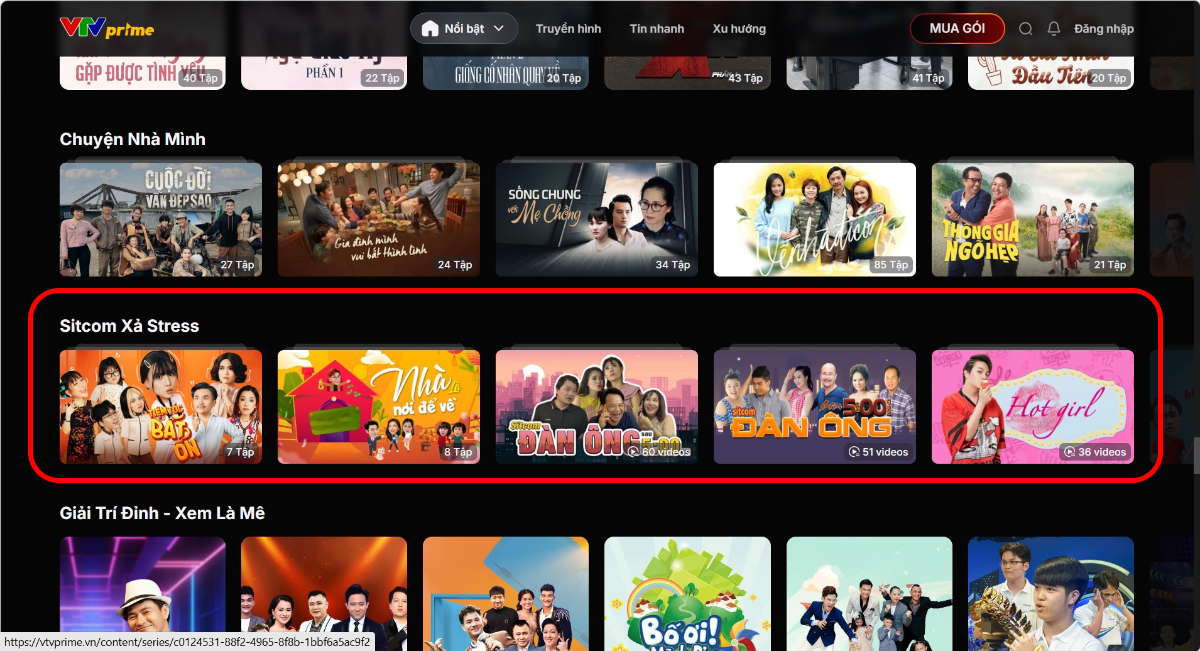
\includegraphics[width=0.6\textwidth]{./vtvprime-product-research-imgs/image1.drawio.png}
  \end{center}
\end{itemize}

\subsubsection{Ưu điểm 2: Lịch phát sóng có hiển thị và sắp xếp theo timeline:}

\begin{itemize}
  \item \textbf{Phân tích}: Khi mở một kênh, lịch phát sóng hiển thị kế bên video đang phát và chứa các thông tin như tên chương trình, thời gian bắt đầu và kết thúc của một chương trình.
  \item \textbf{Nguyên tắc liên quan}: Recognition \& Recall.
  \item \textbf{Ví dụ cụ thể}:
  \begin{quote}
    Người dùng A muốn biết xem kênh họ đang chọn vào lúc 19h00' sẽ phát chương trình nào. Họ chỉ cần liếc mắt qua phải là thấy ngay sắp tới, vào lúc 19h00', sẽ có chương trình thời sự.
  \end{quote}
  \begin{center}
    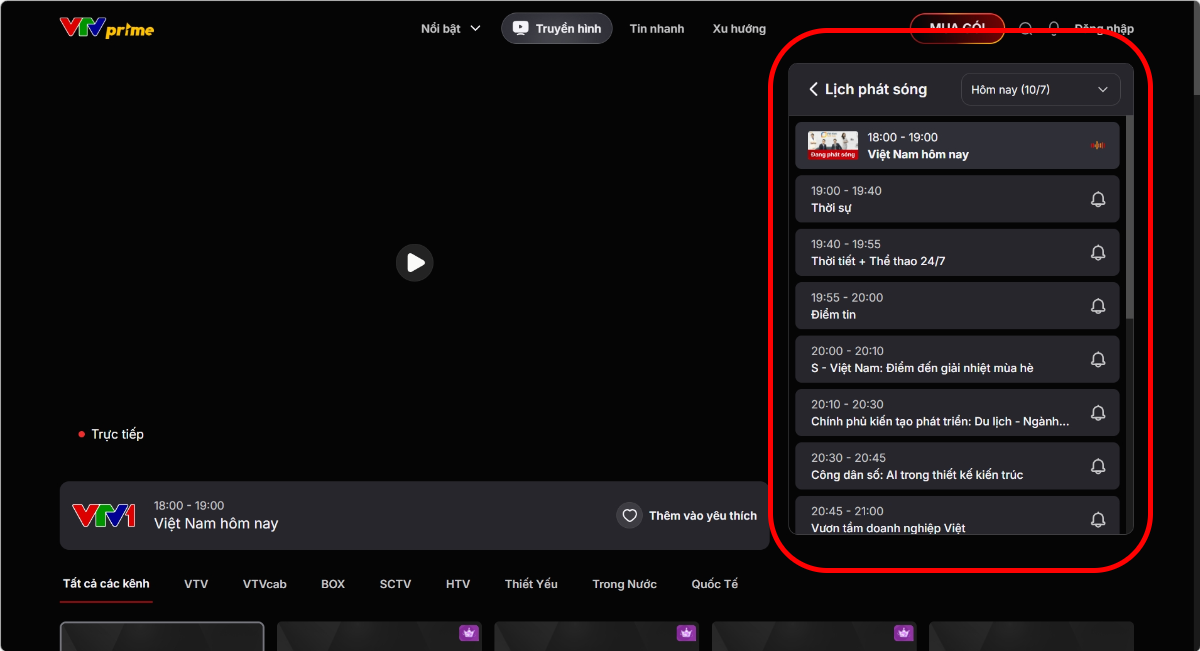
\includegraphics[width=0.6\textwidth]{./vtvprime-product-research-imgs/image2.drawio.png}
  \end{center}
\end{itemize}

\subsubsection{Ưu điểm 3: Pattern giống nhau giữa các carousel}

\begin{itemize}
  \item \textbf{Phân tích}: Các carousel đều dùng chung pattern: Mỗi carousel chứa một heading H2, cạnh bên là nút ``Xem tất cả'', theo sau là các card có liên quan với nhau, giúp người dùng dễ dự đoán cách tương tác mà không cần học lại. Đây là internal consistency giúp người dùng nhanh chóng hiểu được cấu trúc tổng thể, từ đó dễ dàng khám phá nội dung mới mà không gặp trở ngại.
  \item \textbf{Nguyên tắc liên quan}: Consistency, Memorability.
  \item \textbf{Ví dụ cụ thể}:
  \begin{quote}
    Người dùng A đang lướt trang web VTVPrime và thấy mục ``Phim Hay Không Thể Bỏ Lỡ'' có thể cuộn ngang được. Bên trong nó chứa các card đại diện cho các phim mà trang web đề xuất là ``Hay''. Tiếp theo, A lướt xuống và thấy có mục ``Nam Thần Đốn Tim'' có cấu trúc tương tự như mục ``Phim Hay Không Thể Bỏ Lỡ''. Nhờ vậy họ tự khắc suy ra rằng ``Trong mục này có nhiều phim, phim nào cũng có những diễn viên điển trai, tôi có thể scroll sang ngang để xem nhiều hơn!''.
  \end{quote}
  \begin{center}
    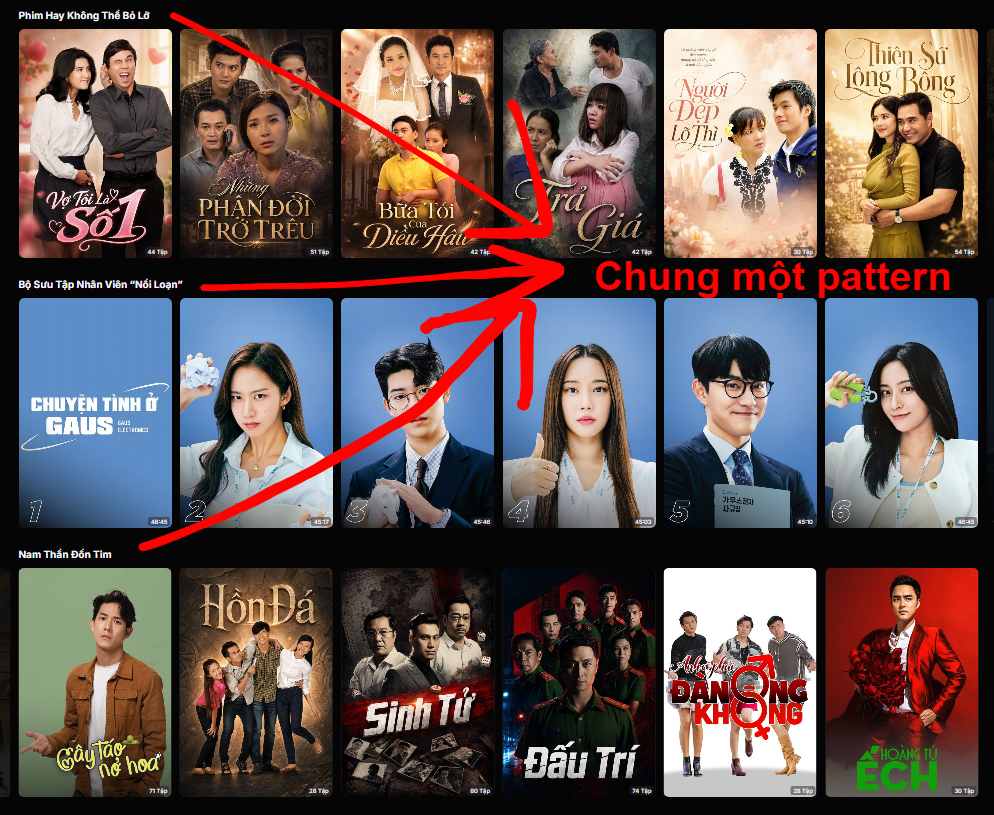
\includegraphics[width=0.6\textwidth]{./vtvprime-product-research-imgs/image3.drawio.png}
  \end{center}
\end{itemize}

\subsubsection{Ưu điểm 4: Các trạng thái ``Đang phát'', ``Sắp phát sóng'' được thể hiện rõ ràng}

\begin{itemize}
  \item \textbf{Phân tích}: Ở trạng thái ``Đang phát'', badge có nền đỏ và trong mô tả của đoạn video sẽ hiển thị thời gian diễn ra video đó. Ở trạng thái ``Sắp phát sóng'' thì badge có nền trắng kèm theo thông tin về thời gian phát sóng, ngày phát sóng. Chính vì vậy mà người xem không phải nhớ nhiều về thời gian họ cần chờ đợi để đón xem video. Lỡ như họ có quên mất và bỏ lỡ phần đầu của một video, thanh tiến trình nhỏ dưới mỗi card cũng sẽ cho biết họ có bỏ lỡ phần hay của video hay không(thường là phần giữa của video, bởi vì khúc đầu thường sẽ giới thiệu nhiều hơn). Nếu bỏ lỡ, họ chỉ việc xem lại sau là được.
  \item \textbf{Nguyên tắc liên quan}: Visibility.
  \item \textbf{Ví dụ cụ thể}:
  \begin{quote}
    Người dùng A mở VTVprime và thấy chương trình ``Genesis Scottish Open | Ngày 2'' đang được gắn badge ``Đang phát'' màu đỏ. Ngoài trạng thái phát trực tiếp, thanh tiến trình bên dưới thẻ nội dung cho biết chương trình đã diễn ra được một phần. Ban đầu, A cũng tò mò muốn xem, nhưng sau khi thấy thanh tiến trình chạy được hơn phân nửa, A quyết định xem sau thay vì loay hoay click vào video, đợi video load xong rồi mới biết video đang ở phút thứ mấy.
  \end{quote}
  \begin{center}
    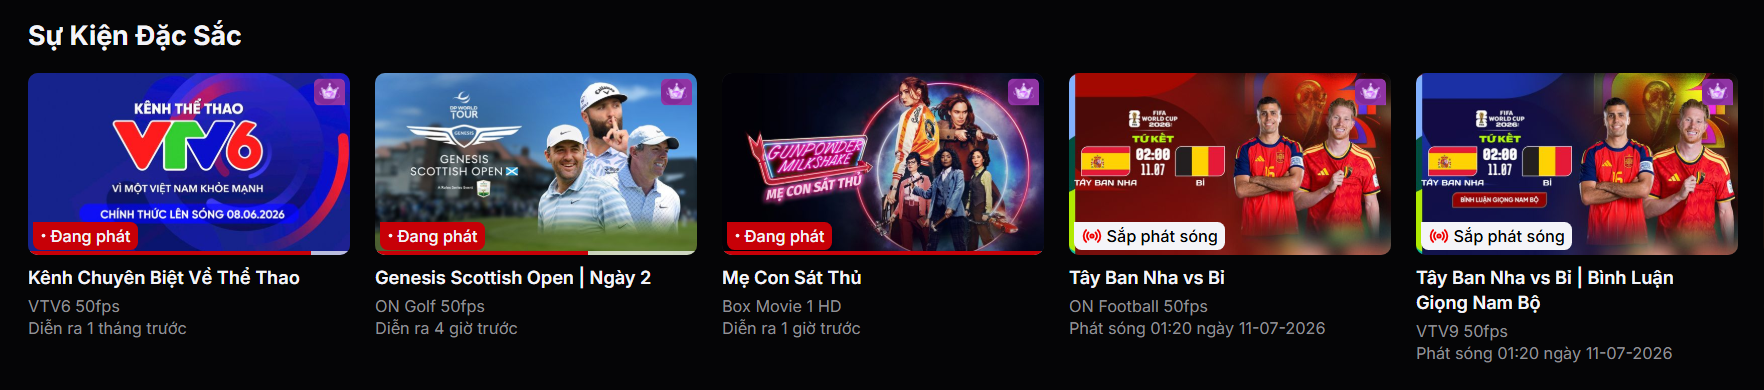
\includegraphics[width=0.6\textwidth]{./vtvprime-product-research-imgs/image4.png}
  \end{center}
\end{itemize}

\subsubsection{Ưu điểm 5: Nhiều thành phần trong giao diện trang web có sử dụng các ``hint'' để người dùng biết cách tương tác với trang web sao cho phù hợp.}

\begin{itemize}
  \item \textbf{Phân tích}: Mỗi card trong trang có hiệu ứng hover nhẹ khi di chuột vào, báo hiệu cho người dùng rằng đây là phần tử có thể click được. Nút ``Xem tất cả \ensuremath{\rangle}'' sử dụng ký hiệu mũi tên (\ensuremath{\rangle}) gợi ý điều hướng sang trang mới. Mũi tên carousel trái/phải gợi ý có thể cuộn ngang để xem thêm nội dung.
  \item \textbf{Nguyên tắc liên quan}: Affordances \& Natural Mapping.
  \item \textbf{Ví dụ cụ thể}:
  \begin{quote}
    Người dùng A từ bé đã thấy ba mẹ của mình lúc chở mình đi học luôn bật xi nhan trái để rẽ trái và bật xi nhan phải để rẽ phải. Dựa vào kinh nghiệm nhiều năm tham gia giao thông như thế, A nhìn vào trang web và biết ngay rằng chỉ cần click vào nút mũi tên phải thì những nội dung bên phải của A sẽ hiện ra, giống hệt như lúc rẽ phải thì sẽ thấy được những khung cảnh ở con đường bên tay phải vậy.
  \end{quote}
  \begin{center}
    \includegraphics[width=0.6\textwidth]{image.png}
  \end{center}
\end{itemize}

\subsubsection{Ưu điểm 6: VTVPrime sử dụng các banner cỡ lớn cho các nội dung quan trọng}

\begin{itemize}
  \item \textbf{Phân tích}: VTVPrime tận dụng metaphor là các banner ở ngoài đường phố để đưa vào trang web của mình, nhấn mạnh những nội dung nổi bật, những nội dung mà họ cho rằng nhiều người dùng sẽ muốn xem. Tính chất chung của banner trong thế giới thật và banner trong trang web là: Chúng đều có kích thước lớn, dễ nhận thấy, hình ảnh thu hút và thông tin súc tích nhưng mang tính kêu gọi sự quan tâm.
  \item \textbf{Nguyên tắc liên quan}: Mental model \& Metaphor.
  \item \textbf{Ví dụ cụ thể}:
  \begin{quote}
    Đây là một banner đường phố. Thông điệp ``Fashion Never Sleep'' tuy ngắn gọn nhưng mang hàm ý kêu gọi mạnh mẽ ``Bạn có thể ngủ, nhưng ngủ dậy nhớ cập nhật những trend hot về thời trang!''. Cái hay ở đây chính là việc kết hợp giữa khẳng định chắc nịch ``NEVER SLEEP'' và những tông màu gần màu đỏ(mắt người nhạy hơn đối với những màu trong dải màu đỏ), khiến cho người dùng có cảm giác như họ phải vào trang fashion.com ngay bên dưới để đọc thêm ngay.
  \end{quote}
  \begin{center}
    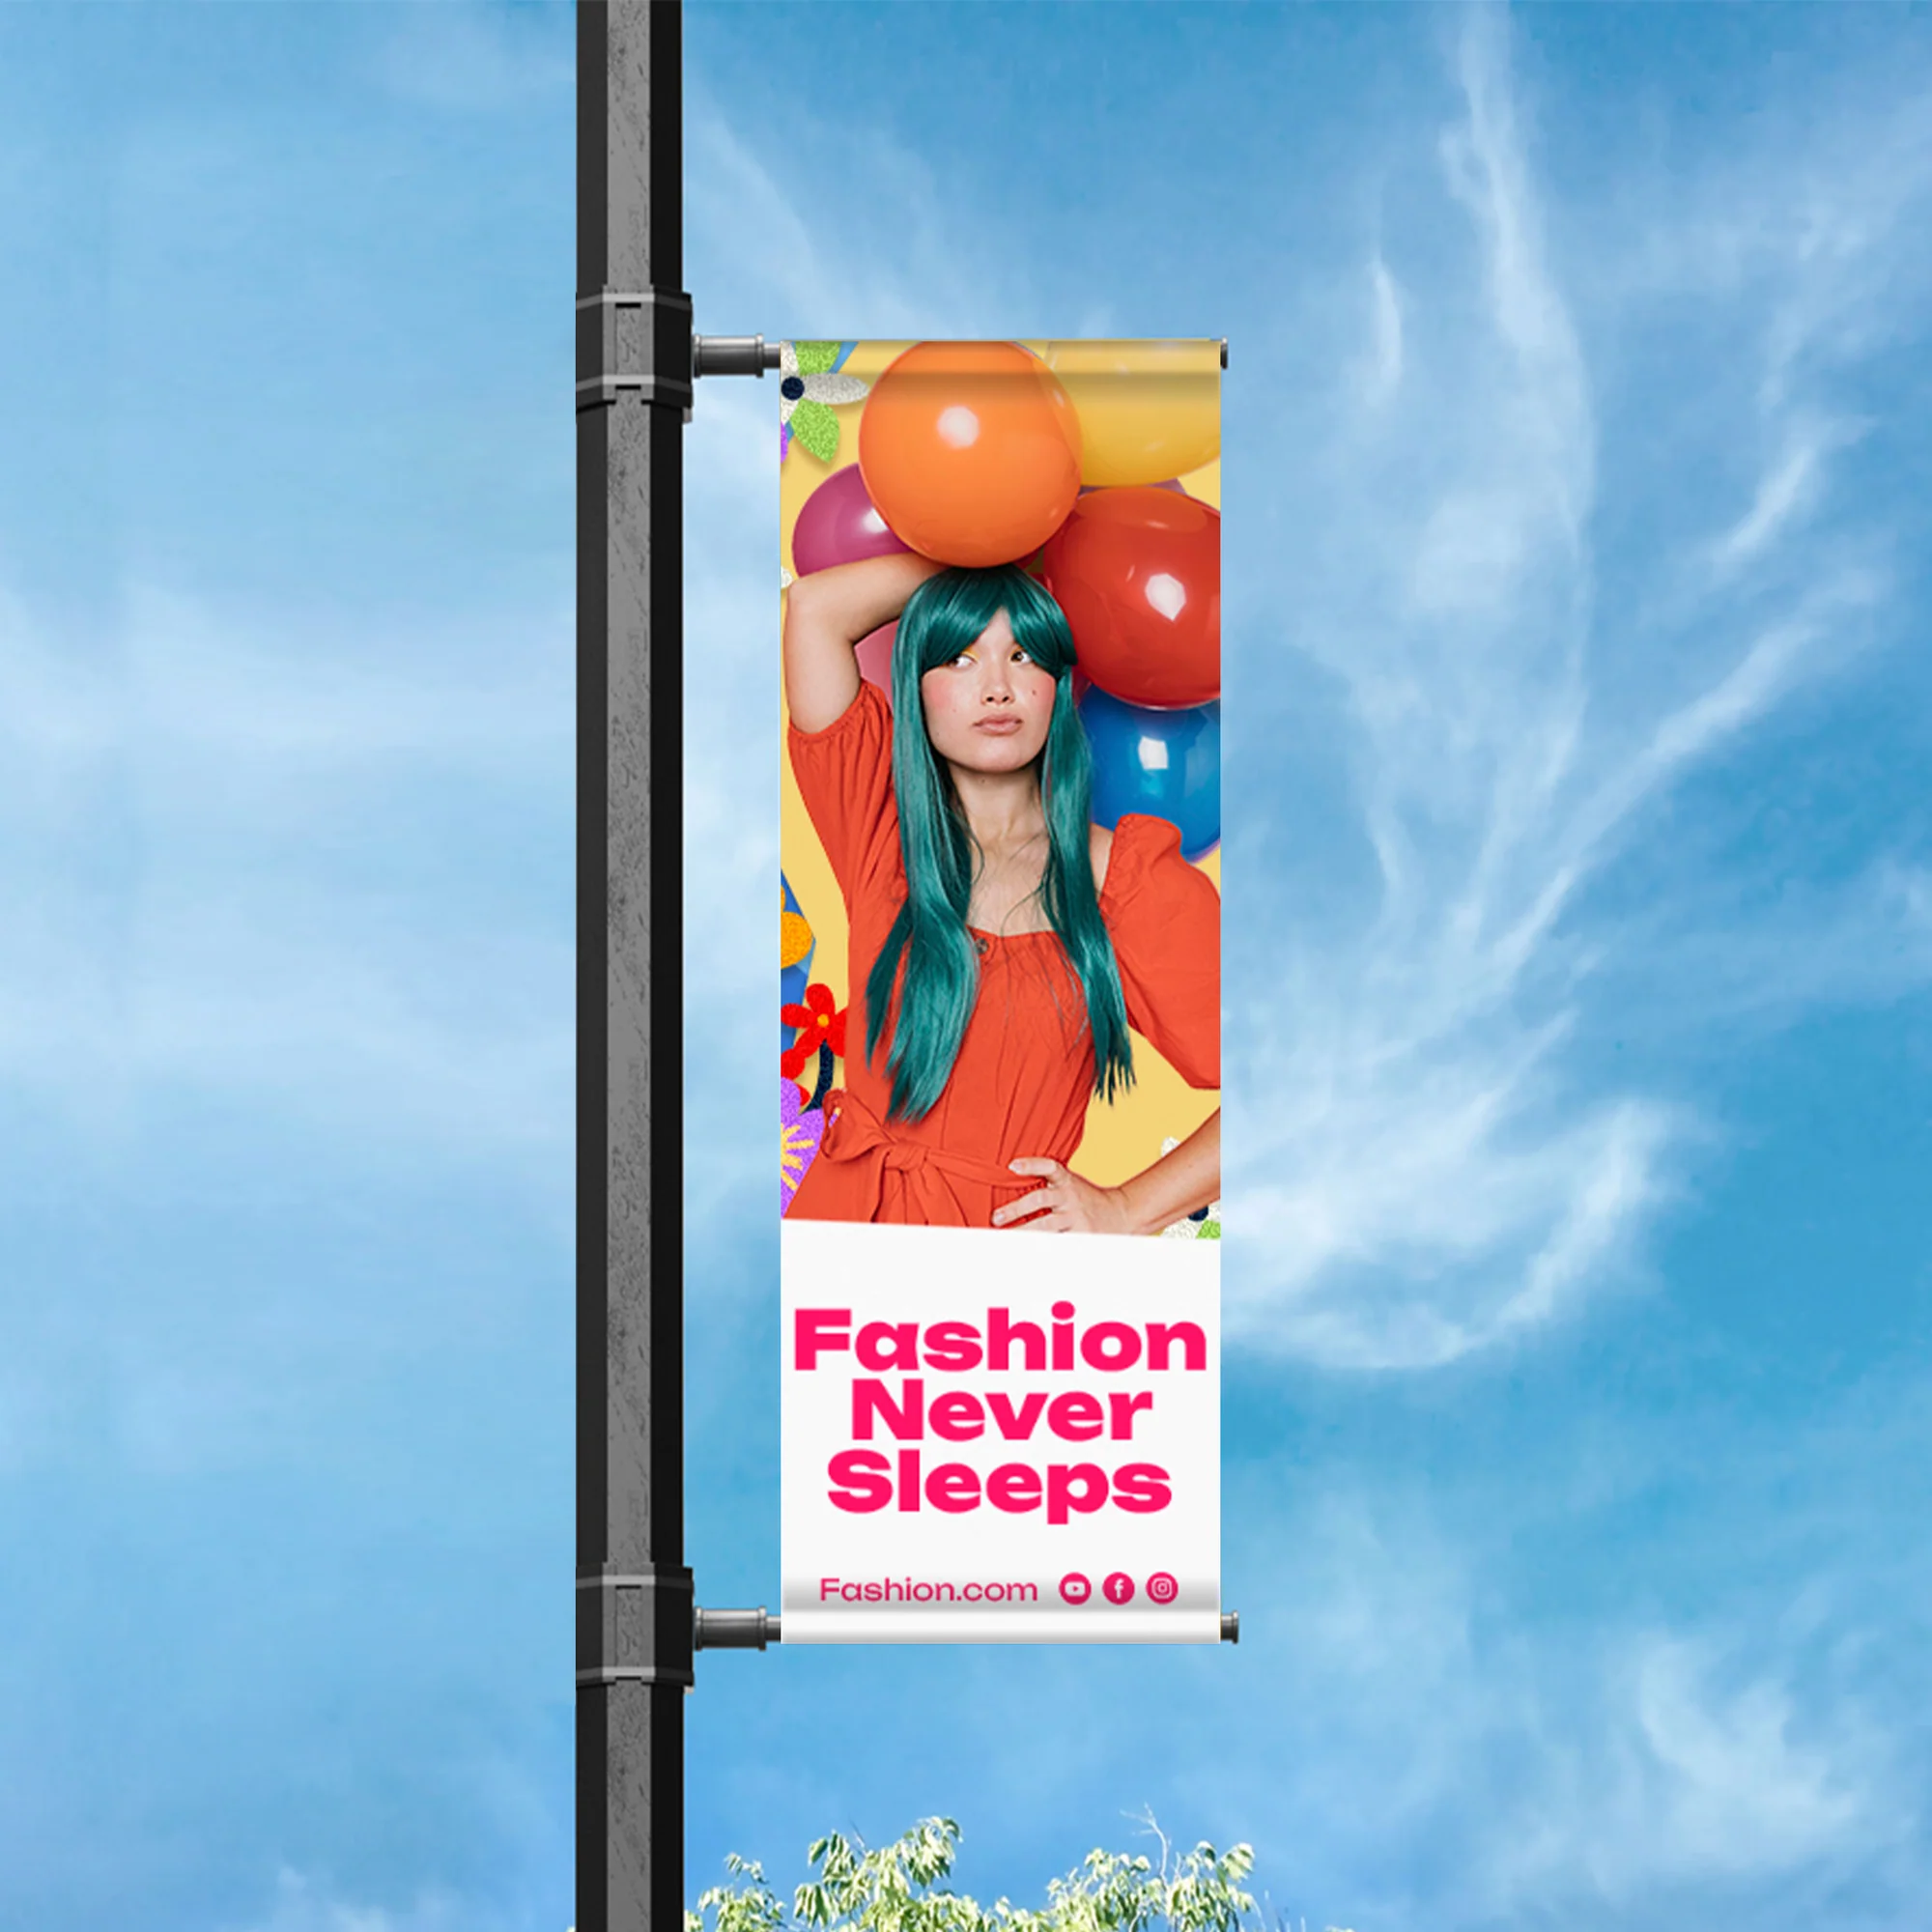
\includegraphics[width=0.6\textwidth]{./vtvprime-product-research-imgs/image7.png}
  \end{center}

  \begin{quote}
    Đây là một banner trong trang VTVPrime. Cả hình ảnh và nội dung chữ viết trên banner này đều kích thích những ham muốn vật chất của con người: Từ hình ảnh điện thoại, xe,\ldots cho đến dòng chữ tô đỏ ``500 triệu đồng'', khiến cho người dùng phải tò mò và click vào dòng chữ ``Xem ngay'' trên banner này.
  \end{quote}
  \begin{center}
    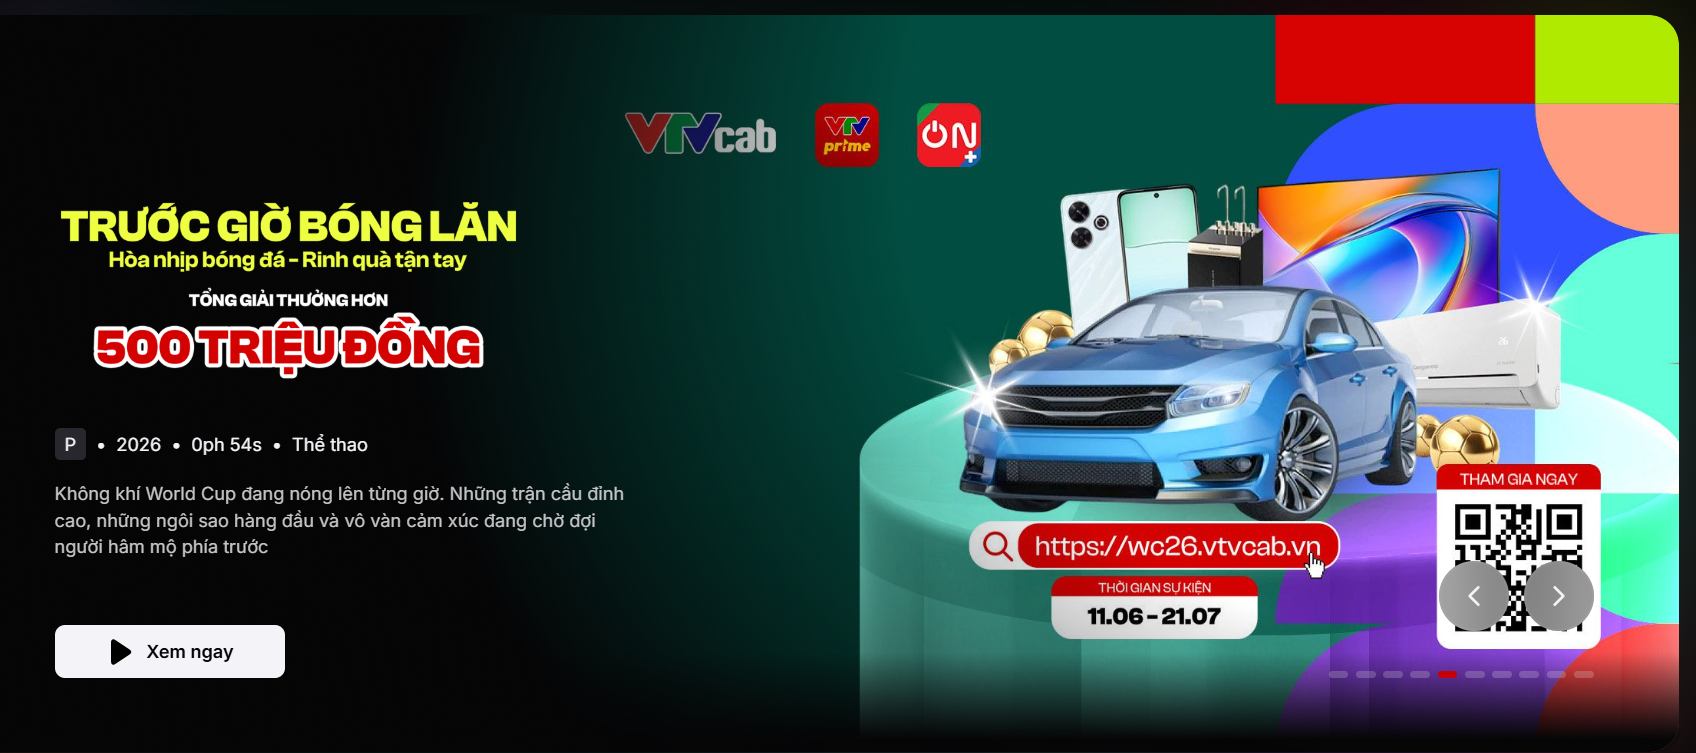
\includegraphics[width=0.6\textwidth]{./vtvprime-product-research-imgs/image8.png}
  \end{center}

  \begin{quote}
    Đây là một banner khác trong trang. Banner này sử dụng hình ảnh của những người nổi tiếng: Lionel Messi(Hoạt động 22 năm, 500M+ followers trên Instagram), Cristiano Ronaldo(Hoạt động 24 năm, 600M+ followers trên Instagram),\ldots để thu hút lượng fan khổng lồ của họ.
  \end{quote}
  \begin{center}
    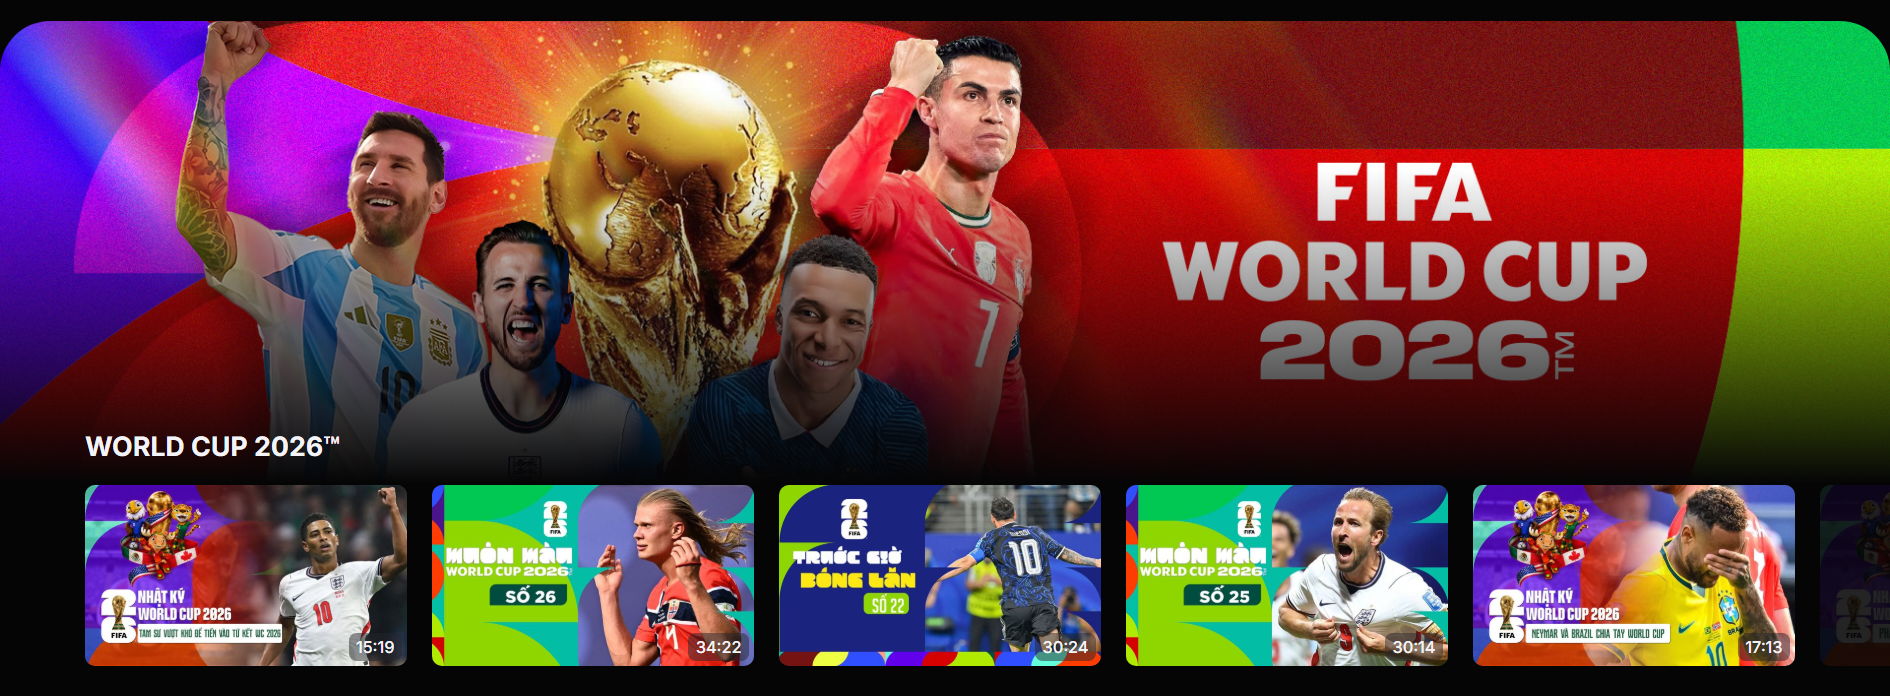
\includegraphics[width=0.6\textwidth]{./vtvprime-product-research-imgs/image9.png}
  \end{center}
\end{itemize}

\subsubsection{Ưu điểm 7: Sử dụng metaphor ``túi đựng tài liệu'' cho các phim bộ}

\begin{itemize}
  \item \textbf{Phân tích}: VTVPrime sử dụng các card có dạng nhiều lớp chồng lên nhau như thế một túi đựng tài liệu để nói với người dùng rằng: Trong một card này có nhiều tập phim chứ không phải chỉ là một live video duy nhất. Ngoài ra, số tập cũng được hiển thị ở góc dưới bên phải của mỗi card một cách rõ ràng, không cần phải click vào rồi đếm thủ công từng tập.
  \item \textbf{Nguyên tắc liên quan}: Mental Model \& Metaphor, Visibility.
  \item \textbf{Ví dụ cụ thể}:
  \begin{quote}
    Đây là các card tượng trưng cho phim bộ.
  \end{quote}
  \begin{center}
    
\includegraphics[width=0.6\textwidth]{./vtvprime-product-research-imgs/image10.png}
  \end{center}

  \begin{quote}
    Mỗi card có nhiều lớp chồng lên nhau.
  \end{quote}
  \begin{center}
    
\includegraphics[width=0.6\textwidth]{./vtvprime-product-research-imgs/image11.drawio.png}
  \end{center}

  \begin{quote}
    Không như card của video bình thường.
  \end{quote}
  \begin{center}
    
\includegraphics[width=0.6\textwidth]{./vtvprime-product-research-imgs/image12.png}
  \end{center}
\end{itemize}

\subsubsection{Ưu điểm 8: Cơ chế cuộn vô tận (infinite scroll) khuyến khích khám phá nội dung}

\begin{itemize}
  \item \textbf{Phân tích HCI}: Trang chủ VTVPrime sử dụng cơ chế infinite scroll --- nội dung liên tục được load thêm khi người dùng kéo xuống mà không có điểm dừng cố định. Đối với một nền tảng xem phim/truyền hình, đây là thiết kế phù hợp vì người dùng không cần nhớ rõ từng bộ phim hay chương trình đã xuất hiện, nên việc có nhiều chunk trên cùng một trang cũng không quá ảnh hưởng tới họ. Hơn nữa, cơ chế này khiến người dùng dành nhiều thời gian hơn trên trang web, và trong quá trình lướt, những nội dung nổi bật nhất (banner lớn, thumbnail thu hút, tiêu đề ấn tượng) sẽ được não bộ ghi nhớ. Số lượng nội dung gây ấn tượng với người dùng tăng lên đồng nghĩa với việc thời gian người dùng bỏ ra để xem trang web cũng tăng lên. Khi đó, VTVPrime sẽ trở thành một phần không thể thiếu trong cuộc sống của họ, buộc họ phải gia hạn gói cước mỗi khi hết hạn.
  \item \textbf{Nguyên tắc liên quan}: Attention \& Cognitive Load.
  \item \textbf{Ví dụ cụ thể}: Người dùng A mở VTVPrime vào tối thứ Bảy, không có ý định xem gì cụ thể --- chỉ muốn ``lướt xem có gì hay''. Nhờ infinite scroll, A cuộn liên tục qua hàng chục carousel: ``Phim Hay Không Thể Bỏ Lỡ'', ``Nam Thần Đốn Tim'', ``Sitcom Xả Stress''\ldots Lướt sâu xuống dưới, A tình cờ thấy carousel ``Phá Đảo Kỳ Thi Tốt Nghiệp THPT'' --- nội dung ôn tập kiến thức THPT mà A không hề biết VTVPrime có --- nếu trang web dùng pagination, A có lẽ đã dừng lại ở ``Trang 1'' và không bao giờ biết đến nội dung này. Cuối phiên, A nhớ rõ 2--3 bộ phim nổi bật nhất mà mình đã thấy, và quyết định xem một trong số đó. Nếu dùng pagination, A sẽ thấy ít nội dung hơn trong cùng thời gian, xác suất ``tình cờ phát hiện'' nội dung mới giảm đáng kể.
\end{itemize}

\subsection{Nhược điểm}

\subsubsection{Nhược điểm 1: Không có tên nội dung hay mô tả ngắn cho nhiều thumbnail}

\begin{itemize}
  \item \textbf{Hiện trạng}: Trong nhiều carousel, mỗi card thumbnail chỉ hiển thị thời lượng video mà không có tên nội dung hoặc mô tả ngắn bên dưới. Người dùng phải click vào, sau đó đợi chuyển trang thì mới biết đó là video gì. Trong khi đó, một vài carousel khác lại làm tốt điều này. Đây là sự thiếu tính nhất quán trên trang web, cũng như thiếu sự thể hiện những thông tin cần thiết.
  \item \textbf{Nguyên tắc liên quan}: Visibility, Consistency.
  \item \textbf{Ví dụ cụ thể}:
  \begin{quote}
    Người dùng A muốn tìm video highlight trận ``Pháp vs Maroc'' đã diễn ra. Trong mục ``Highlights World Cup 2026\texttrademark{}'', tất cả card đều hiển thị ảnh thumbnail nhỏ và thời lượng, nhưng không có tiêu đề. Giả sử A không phải là một người xem World Cup thường xuyên. Khi đó, trừ khi A vô tình nhận diện được khuôn mặt của một cầu thủ bất kì nào đó trong một thumbnail nào đó và biết chính xác cầu thủ đó ở đội nào, A phải click vào từng thumbnail một trong carousel cho đến khi thông tin chi tiết lúc chuyển trang có tiêu đề chứa từ khóa ``Pháp'' và ``Ma Rốc''. So sánh với YouTube: Cũng thể hiện các thumbnail card, nhưng YouTube hiển thị \textbf{title + tên kênh + lượt xem + thời gian đăng tải} bên dưới mỗi thumbnail. Nhờ vậy, người dùng nhận ra ngay nội dung của video là gì, mức độ phổ biến của video như thế nào trước cả khi họ di chuyển con trỏ chuột vào thumbnail của video đó. Ở đây, đội ngũ thiết kế của VTVPrime có sử dụng hình ảnh các lá cờ và tên nước của mỗi đội trong thumbnail. Nhưng lỡ như một ngày nào đó trong tương lai, họ không thiết kế thumbnail theo kiểu đó thì sao?
  \end{quote}
  \begin{center}
    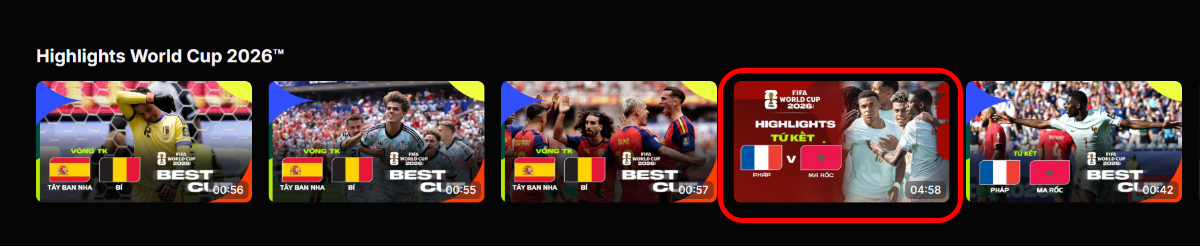
\includegraphics[width=0.6\textwidth]{./vtvprime-product-research-imgs/image15.drawio.png}
  \end{center}

  \begin{quote}
    Sau khi xem xong highlight trận tứ kết giữa Pháp và Ma Rốc, người dùng trở về trang chủ và tiếp tục lướt tiếp trang web. Khi thấy phần thông tin về NSƯT Hoàng Hải, họ sẽ thắc mắc ``Tại sao ở chỗ này, tôi có thể thấy rõ tên của các bộ phim, nhưng ở phần highlight World Cup 2026 ban nãy thì tôi lại không thấy?''. Người dùng sẽ cảm thấy đôi phần không hài lòng khi chất lượng phục vụ họ trên trang web không ổn định.
  \end{quote}
  \begin{center}
    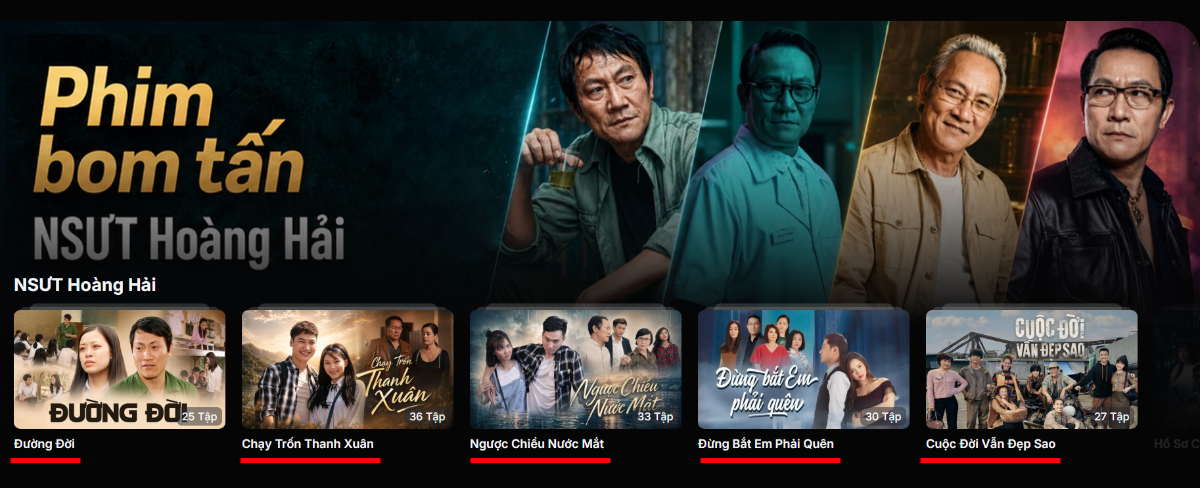
\includegraphics[width=0.6\textwidth]{./vtvprime-product-research-imgs/image16.drawio.png}
  \end{center}

  \item \textbf{Đề xuất hướng khắc phục}: Thêm tiêu đề ngắn bên dưới mỗi thumbnail (``Pháp vs Maroc - Highlight'', ``Bàn thắng đẹp nhất ngày'',\ldots).
\end{itemize}

\subsubsection{Nhược điểm 2: Mũi tên carousel quá nhỏ và đặt sai vị trí --- vi phạm Fitts's Law}

\begin{itemize}
  \item \textbf{Phân tích}: Một nguyên tắc quan trọng sinh từ Fitts's Law là screen edge effect: khi mục tiêu nằm ở mép màn hình, chiều rộng hiệu dụng của nó trở nên vô tận vì cursor sẽ dừng lại ở rìa screen --- người dùng không cần canh position chính xác, chỉ cần kéo chuột hết cỡ về phía đó là trúng. Đúng lý tưởng, mũi tên carousel nên đặt ở sát mép màn hình (side-edge) với height bằng chiều cao carousel --- tạo thành vùng target khổng lồ, dễ click nhất có thể. Tuy nhiên, VTVPrime đặt mũi tên bên trong carousel, có kích thước nhỏ, trên nền tối cùng tông màu nên vừa không tận dụng lợi thế screen edge, vừa thiếu độ tương phản để nhận diện nhanh. Người dùng phải nhìn kỹ rồi di chuột chính xác mới click được --- tăng thời gian tương tác.
  \item \textbf{Nguyên tắc liên quan}: Efficiency / Fitts's Law.
  \item \textbf{Ví dụ cụ thể}:
  \begin{quote}
    Người dùng A muốn cuộn carousel ``Nội Dung World Cup 2026\texttrademark{} Mới Nhất'' sang phải để xem thêm nội dung. Mũi tên phải nhỏ, nằm bên trong carousel trên nền tối nên bị hòa lẫn vào background, người dùng phải nhìn kỹ rồi di chuột chính xác vào đúng vùng nhỏ đó mới click được. So sánh lý tưởng: mũi tên đặt ở sát mép phải màn hình, có height bao phủ toàn bộ chiều cao carousel \ensuremath{\rightarrow} người dùng chỉ cần kéo chuột hết cỡ sang phải là click trúng. Khoảng cách di chuyển (d) giảm đáng kể và kích thước mục tiêu (s) tăng lên gấp nhiều lần nên theo Fitts's Law, thời gian tương tác giảm mạnh.
  \end{quote}
  \begin{center}
    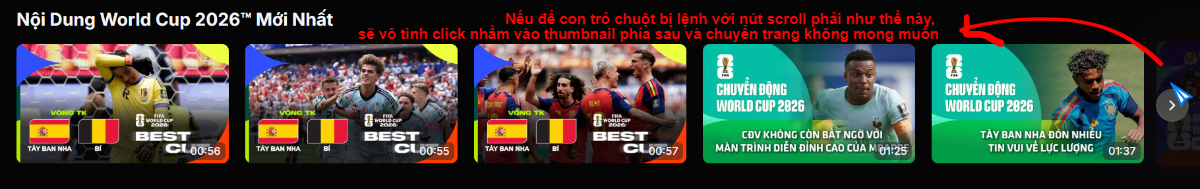
\includegraphics[width=0.6\textwidth]{./vtvprime-product-research-imgs/image17.drawio.png}
  \end{center}
  \item \textbf{Đề xuất hướng khắc phục}: Đặt mũi tên carousel ở sát mép màn hình trái/phải với height bằng chiều cao carousel. Tăng kích thước vùng click để tận dụng lợi thế screen edge effect.
\end{itemize}

\subsubsection{Nhược điểm 3: Thiếu feedback cho infinite scrolling}

\begin{itemize}
  \item \textbf{Phân tích}: Khi cuộn đến cuối cùng của nội dung trên trang chủ, không có dòng text hay dấu hiệu nào cho biết ``đã hết nội dung'' hoặc ``không còn gì để hiển thị''. Hệ thống chỉ đơn giản là dừng load --- người dùng không biết là do đã hết nội dung thật hay do mạng lag/đang load tiếp. Theo nguyên tắc Feedback, hệ thống cần phản hồi trạng thái sau mỗi hành động của người dùng. Khi thiếu feedback ở trạng thái cuối trang, người dùng rơi vào tình trạng không chắc chắn --- không biết nên chờ thêm hay đã hết, dẫn đến hành vi chờ đợi vô ích hoặc tưởng ứng dụng bị lỗi.
  \item \textbf{Nguyên tắc liên quan}: Feedback.
  \item \textbf{Ví dụ cụ thể}:
  \begin{quote}
    Người dùng cuộn đến cuối trang chủ, trang dừng load. Họ chờ 5-10 giây vì nghĩ mạng chậm, nhưng thực tế không còn gì nữa. Sau vài lần như vậy họ mới hiểu ra, nhưng mỗi lần vẫn phải mất thời gian ``đoán'' trạng thái hệ thống.
  \end{quote}
  \begin{center}
    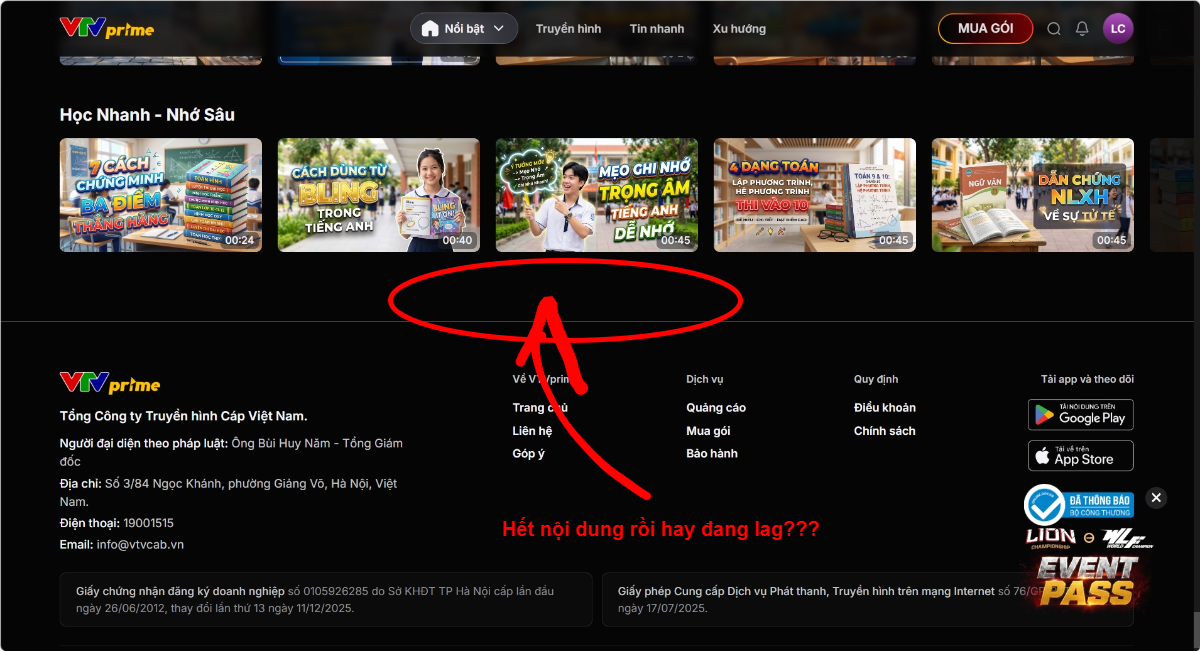
\includegraphics[width=0.6\textwidth]{./vtvprime-product-research-imgs/image18.drawio.png}
  \end{center}
  \item \textbf{Đề xuất hướng khắc phục}: Thêm dòng text như ``Đã hiển thị tất cả nội dung''.
\end{itemize}

\subsubsection{Nhược điểm 4: Nút ``Xem tất cả \ensuremath{\rangle}'' không nhất quán giữa các section}

\begin{itemize}
  \item \textbf{Phân tích}: Internal consistency yêu cầu các thành phần \textbf{cùng chức năng} phải hoạt động giống nhau ở mọi nơi. Các carousel trong trang có chức năng hiển thị một phần thông tin nhưng chỉ một số carousel có nút bấm ``Xem tất cả \ensuremath{\rangle}'' (cho phép xem toàn bộ thông tin), nhiều carousel khác thì không. Điều này phá vỡ pattern recognition: Người dùng học được pattern ``heading + Xem tất cả \ensuremath{\rangle}'' ở carousel đầu tiên. Họ kỳ vọng carousel sau cũng có, nhưng thật ra là không.
  \item \textbf{Nguyên tắc liên quan}: Consistency.
  \item \textbf{Ví dụ cụ thể}:
  \begin{quote}
    Người dùng A thấy carousel ``World Cup 2026\texttrademark{}'' có nút ``Xem tất cả \ensuremath{\rangle}'' bên phải, họ click vào và xem được toàn bộ danh sách các video. Tiếp tục lướt xuống, A thấy section ``Muôn Màu World Cup'' cũng là carousel tương tự, kỳ vọng sẽ có ``Xem tất cả \ensuremath{\rangle}'' nhưng không có. A thắc mắc: ``Tại sao section này không có? Vậy mình phải làm sao để xem tất cả các nội dung đây? Chẳng lẽ mình phải lướt hết carousel? Lỡ như carousel này dài quá thì sao? Mình sẽ tốn bao nhiêu thời gian để lướt hết carousel này? Mình có nên lướt tiếp không?\ldots'' \ensuremath{\rightarrow} mất thời gian tìm kiếm và bị bỡ ngỡ.
  \end{quote}
  \begin{quote}
    ``World Cup 2026\texttrademark{}'' có nút ``Xem tất cả''.
  \end{quote}
  \begin{center}
    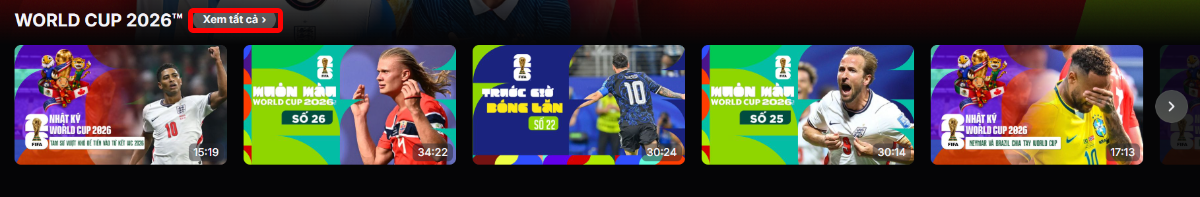
\includegraphics[width=0.6\textwidth]{./vtvprime-product-research-imgs/image19.drawio.png}
  \end{center}
  \begin{quote}
    ``Muôn Màu World Cup'' không có nút này.
  \end{quote}
  \begin{center}
    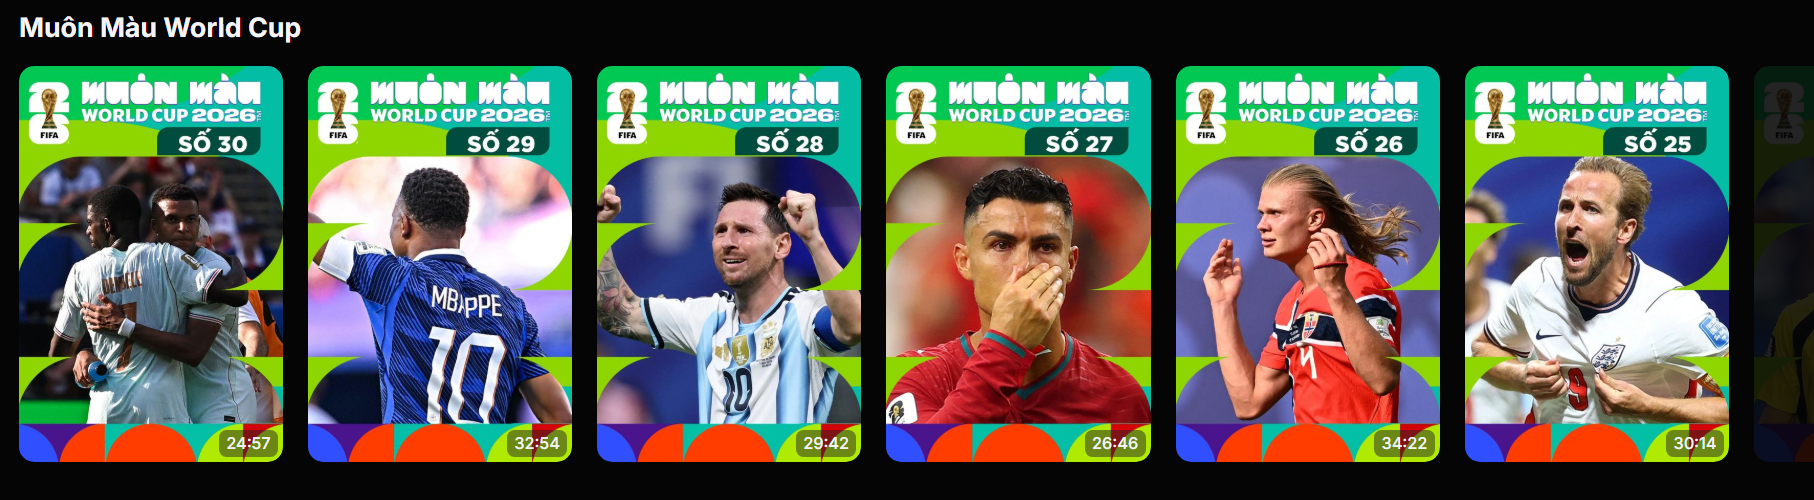
\includegraphics[width=0.6\textwidth]{./vtvprime-product-research-imgs/image20.png}
  \end{center}
\end{itemize}

\subsubsection{Nhược điểm 5: Nhiều ảnh bị để trống alt text --- vi phạm Accessibility}

\begin{itemize}
  \item \textbf{Phân tích HCI}: Tất cả ảnh trên trang web nên có alt text --- thuộc tính mô tả nội dung ảnh cho phần mềm đọc màn hình (screen reader) của người khiếm thị. Khi ảnh để trống alt text, screen reader sẽ bỏ qua hoàn toàn, người dùng khiếm thị không biết ảnh đó chụp gì. Trên trang chủ VTVPrime, có nhiều ảnh bị để trống alt text hoặc có nhưng vô dụng(Ví dụ: alt=``poster''). Đặc biệt quan trọng với các ảnh thumbnail phim/program vì đây là nội dung chính mà người dùng cần nhận diện để quyết định xem hay không.
  \item \textbf{Nguyên tắc liên quan}: Accessibility / Inclusive Design.
  \item \textbf{Ví dụ cụ thể}:
  \begin{quote}
    Một người khiếm thị sử dụng phần mềm đọc màn hình truy cập VTVPrime. Khi cuộn qua các carousel, screen reader đọc: ``heading: Phim Hay Không Thể Bỏ Lỡ. image. image. image. heading: Nam Thần Đốn Tim. image. image. image\ldots'' --- người dùng nghe toàn là ``image'' mà không biết ảnh nào chụp phim gì, vì alt text bị bỏ trống. Nếu alt text được điền đúng (vd: alt=``Poster phim Thỏ Peter - 10 tập, thể loại phiêu lưu''), screen reader sẽ đọc: ``image: Poster phim Thỏ Peter - 10 tập, thể loại phiêu lưu'' \ensuremath{\rightarrow} người dùng biết ngay nội dung mà không cần click vào.
  \end{quote}
  \item \textbf{Đề xuất hướng khắc phục}: Thêm alt text có nghĩa cho tất cả 16 ảnh đang để trống trên trang chủ. Alt text nên mô tả ngắn gọn nội dung ảnh, ví dụ: alt=``Poster phim Thỏ Peter'', alt=``Highlight trận Pháp vs Maroc - World Cup 2026''. Không dùng alt text chung chung như alt=``image'' hoặc alt=``photo''.
\end{itemize}

\subsubsection{Nhược điểm 6: Nút ``Xem tất cả'' quá nhỏ và nằm xa vùng tương tác của người dùng}

\begin{itemize}
  \item \textbf{Phân tích}: Nút ``Xem tất cả'' nhỏ, lại luôn show mỗi lần rê chuột vào một card bất kì. Với trường hợp người dùng đang rê chuột vào các card ở phía cuối, khoảng cách d từ card đến nút ``Xem tất cả'' sẽ lớn hơn. Hơn nữa, khi rê chuột ở vị trí cuối, thường là người dùng đang ở trong tâm thế muốn hiện thêm kết quả, vì vậy tần suất họ muốn click vào nút ``Xem tất cả'' sẽ tăng. Số lần click tăng và thời gian tương tác cũng tăng sẽ gây ra độ trễ tích lũy khổng lồ đối với hành vi của người dùng.
  \item \textbf{Nguyên tắc liên quan}: Efficiency / Fitts' Law.
  \item \textbf{Giải pháp đề xuất}: Nhóm nghĩ ra hai giải pháp. Một là đẩy nút ``Xem tất cả'' vào giữa và kéo dài nút ra. Hai là đưa các header vào một khung chứa, có background color và có thể click được. Khi đó, khoảng cách từ mỗi card đến vị trí cần click để xem tất cả kết quả là như nhau và cũng chính là khoảng cách nhỏ nhất.
  \item \textbf{Ví dụ cụ thể}:
  \begin{quote}
    Người dùng A muốn xem tất cả những video liên quan đến WORLD CUP 2026 khi họ đang rê chuột đến video cuối cùng trong carousel. Con chuột của họ đang bị hư, họ phải dùng touchpad trên laptop và ngón tay của họ cũng bị trày xước nhẹ khiến cho việc di chuyển ngón tay trên touchpad cũng hơi khó khăn. Họ thấy nút ``Xem tất cả'' nằm tuốt ở phía bên trái và tuy không thích nhưng vẫn phải chấp nhận việc rê con trỏ chuột đến nút ấy chỉ để phát hiện ra rằng trong danh sách đầy đủ cũng không chứa nội dung nội dung họ quan tâm. Họ cảm thấy khó chịu trong lòng.
  \end{quote}
  \begin{center}
    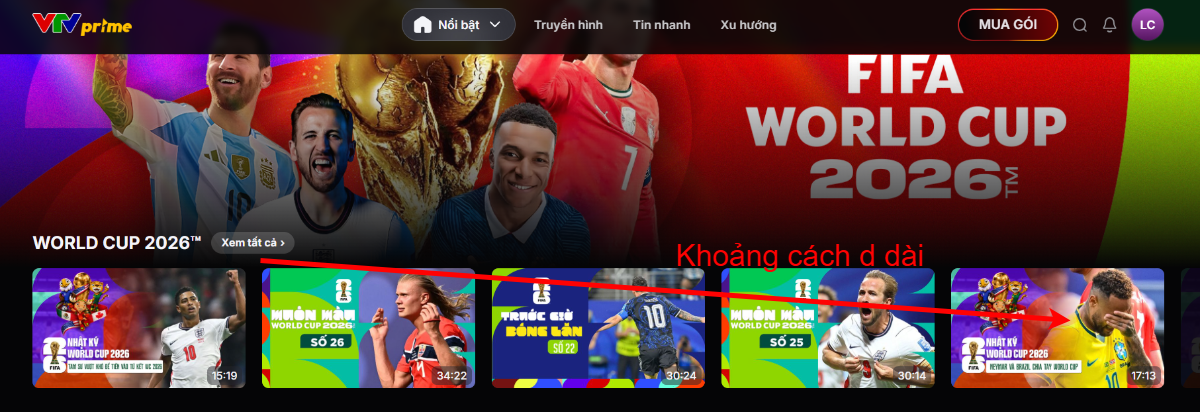
\includegraphics[width=0.6\textwidth]{./vtvprime-product-research-imgs/image5.drawio.png}
  \end{center}
\end{itemize}

\subsubsection{Nhược điểm 7: Định dạng card phim bộ không nhất quán giữa các carousel}

\begin{itemize}
  \item \textbf{Phân tích HCI}: Đều là phim bộ nhưng VTVPrime sử dụng hai định dạng card khác nhau: phần lớn carousel dùng card \textbf{nằm ngang} với metaphor ``túi đựng tài liệu'' (nhiều lớp chồng lên nhau), nhưng một số carousel khác lại dùng card \textbf{dọc} mà không có metaphor này. Theo nguyên tắc \textbf{Internal Consistency}, cùng một loại nội dung (phim bộ) nên có cùng một format trình bày để người dùng nhận ra ngay mà không cần suy luận. Khi định dạng thay đổi đột ngột giữa các carousel, mental model của người dùng bị phá vỡ --- họ đã quen với pattern ``phim bộ = card ngang layers'' ở carousel trước, nhưng carousel sau lại dùng card dọc \ensuremath{\rightarrow} phải học lại pattern mới.
  \item \textbf{Nguyên tắc liên quan}: Consistency (Internal Consistency), Mental Model.
  \item \textbf{Ví dụ cụ thể}:
  \begin{quote}
    Mục ``VTVprime Đề Xuất'' chứa các card phim bộ nằm ngang với nhiều lớp chồng lên nhau (metaphor ``túi đựng tài liệu'') \ensuremath{\rightarrow} người dùng hiểu ``đây là phim bộ''. Nhưng khi cuộn xuống mục ``Phim Hay Không Thể Bỏ Lỡ'' --- cũng là phim bộ --- lại dùng định dạng card dọc, không có layers \ensuremath{\rightarrow} người dùng phải dừng lại nhận diện lại format, mất thời gian thích nghi.
  \end{quote}
  \begin{center}
    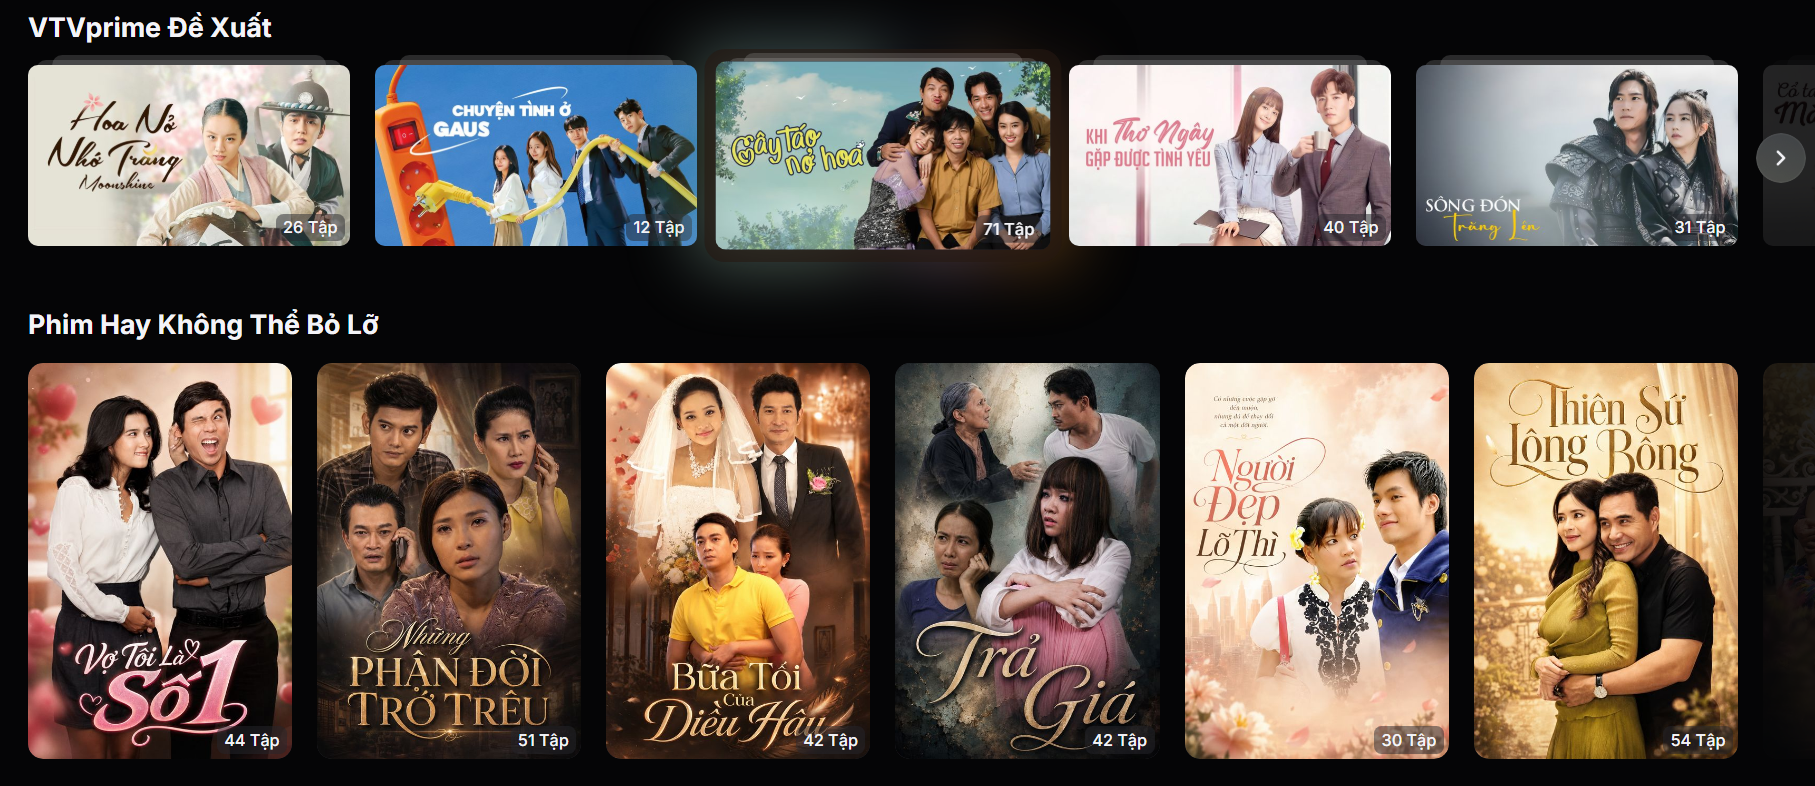
\includegraphics[width=0.6\textwidth]{./vtvprime-product-research-imgs/image13.png}
  \end{center}
\end{itemize}

\subsubsection{Nhược điểm 8: Nút ``Mua gói'' đặt sai vị trí và thiếu feedback sau khi mua}

\begin{itemize}
  \item \textbf{Phân tích}: ``Mua gói'' tuy không phải là một chức năng được sử dụng thường xuyên(người dùng chỉ thanh toán 1 lần cho 1 tuần, 30 ngày,\ldots) nhưng nút bấm này được gom nhóm để nằm sát bên cạnh nút tìm kiếm(một tính năng được dùng thường xuyên). Thậm chí, nút ``Mua gói'' còn to hơn nút tìm kiếm, có màu sắc nổi bật hơn nút tìm kiếm. Ngay cả khi đã mua gói, nút ``Mua gói'' vẫn không biến mất hoặc đổi trạng thái mà vẫn hiển thị ở đó như chưa có gì xảy ra.
  \item \textbf{Nguyên tắc liên quan}: Attention, Feedback.
  \item \textbf{Ví dụ cụ thể}:
  \begin{quote}
    Sau khi người dùng A đăng ký mua gói ``Prime'' trong giao diện mua gói, hệ thống trả về trang chủ. Tuy nhiên, giao diện hầu như không thay đổi, không có phản hồi gì mới, icon của user vẫn giữ nguyên như thể chưa có chuyện gì xảy ra.
  \end{quote}
  \begin{quote}
    Trước và sau khi mua gói đều không đổi:
  \end{quote}
  \begin{center}
    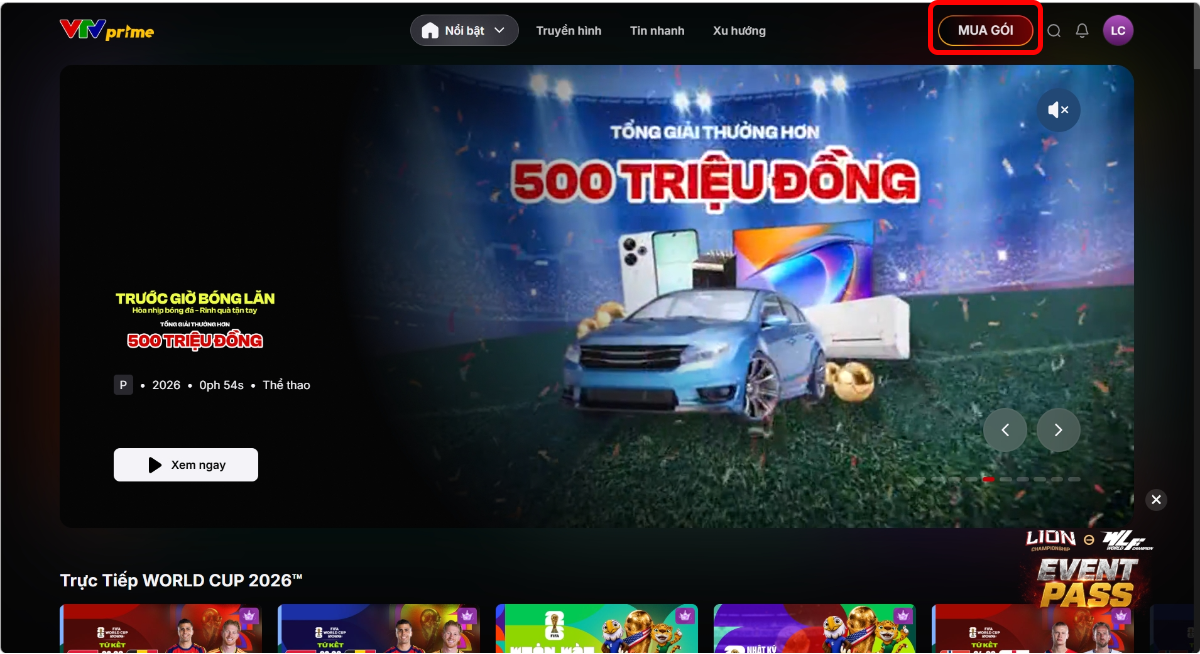
\includegraphics[width=0.6\textwidth]{./vtvprime-product-research-imgs/image14.drawio.png}
  \end{center}
\end{itemize}

\subsubsection{Nhược điểm 9: Giao diện trang mua gói gây nhầm lẫn giữa các gói cước}

\begin{itemize}
  \item \textbf{Phân tích}: Có 4 loại gói cước trong trang ``Mua gói'' của VTVPrime: LION vs WLF, World Cup, Prime, Vinaphone. Nhưng giao diện đăng ký gói cước khiến cho người dùng cảm thấy khó hiểu. Cùng phân tích một số ví dụ bên dưới để làm rõ điều này.
  \item \textbf{Nguyên tắc liên quan}: Visibility, Learnability, Error Prevention.
  \item \textbf{Ví dụ cụ thể}:
  \begin{quote}
    Người dùng A đăng ký mua gói cước Prime thành công với số lượng kênh là 100+ theo như khẳng định trên trang web.
  \end{quote}
  \begin{center}
    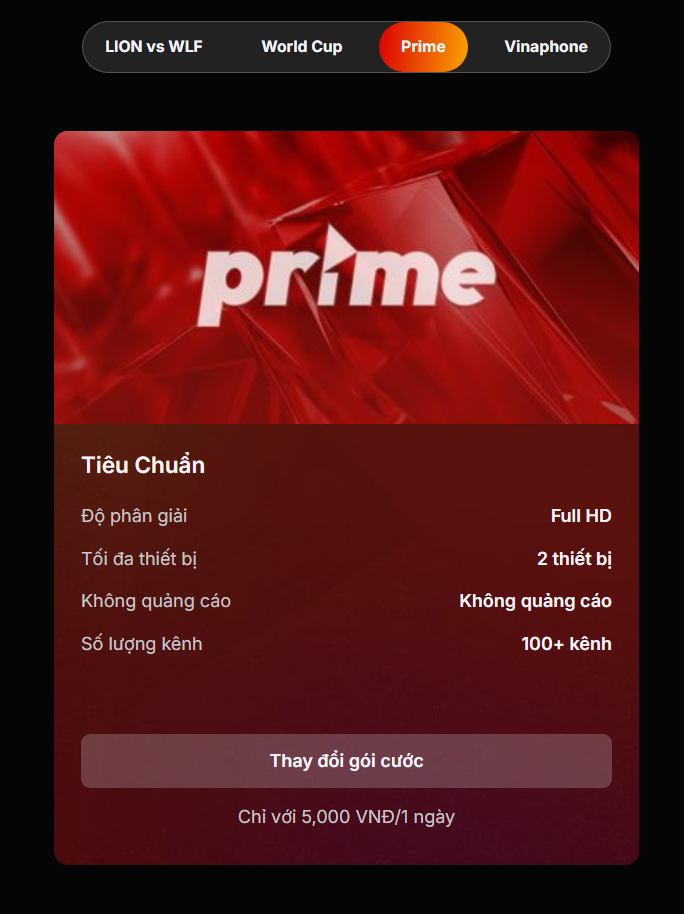
\includegraphics[width=0.6\textwidth]{./vtvprime-product-research-imgs/image21.png}
  \end{center}

  \begin{quote}
    Một khoảng thời gian sau, A vì muốn đăng ký cộng dồn thời lượng sử dụng của cùng gói cước Prime nên A lại truy cập vào trang mua gói. Lúc này, mặc định trang web sẽ hiển thị thông tin của gói đầu tiên từ bên trái - gói LION vs WLF. Tuy nhiên, lúc này vấn đề xuất hiện. A thấy giao diện gói LION vs WLF có nút ``\textbf{Nâng cấp} trải nghiệm'' trong khi quyền lợi ít hơn(chỉ có kênh chiếu ``3 trận LION vs WLF + 7 trận LC33 diễn ra ngày 11/7/2026''). A sẽ thắc mắc ``Tại sao số kênh ít hơn gói hiện tại của mình nhưng lại có nút NÂNG CẤP nhỉ? Vậy là gói này sẽ chứa 100+ kênh trong gói hiện tại của mình VÀ những kênh chiếu các trận đấu diễn ra vào ngày 11/7/2026 hay là chỉ chứa các kênh chiếu các trận đấu này thôi? Nếu cũng là gói 100+ kênh thì tại sao giá lại rẻ hơn? Không lẽ gói này đang giảm giá cho đến ngày 11/7? Mình có nên mua ngay để được cộng dồn thời hạn sử dụng với mức giá rẻ hơn hay không? Mà lỡ không như mình nghĩ, mua gói này xong thì gói kia sẽ bị hủy thì sao?\ldots'' Chỉ cần một suy đoán sai lầm, A sẽ bị mất tiền oan. Giao diện này cực kì không minh bạch đối với một giao diện có liên quan đến vấn đề tiền bạc.
  \end{quote}
  \begin{center}
    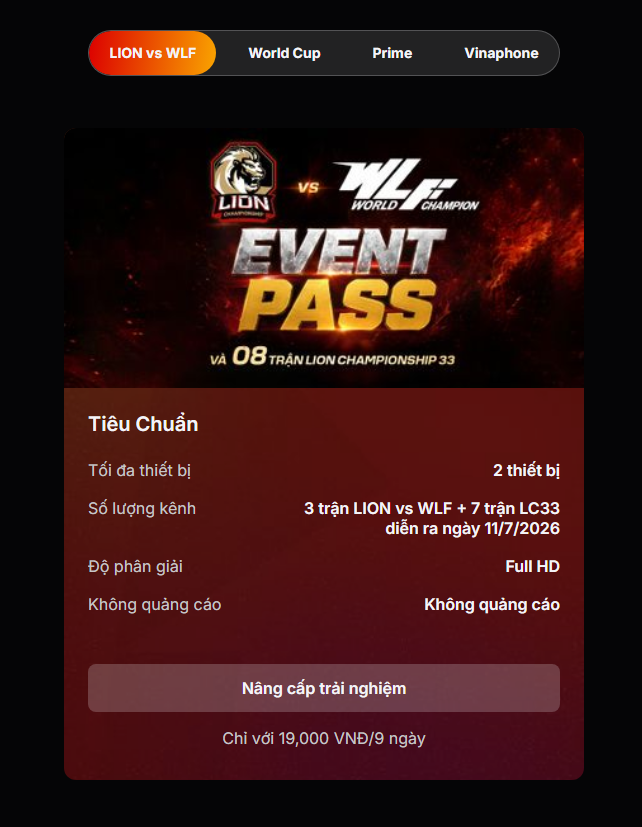
\includegraphics[width=0.6\textwidth]{./vtvprime-product-research-imgs/image22.png}
  \end{center}
\end{itemize}

\subsubsection{Nhược điểm 10: Lịch phát sóng có ký tự ``\textless{}'' vô dụng và các mục đều có dạng nút bấm gây lỗi}

\begin{itemize}
  \item \textbf{Phân tích}: (1) \textbf{Ký tự ``\textless{}'' đặt trước tiêu đề ``Lịch phát sóng''} nhưng nó không có chức năng gì khi click vào. Trong giao diện web, ký tự ``\textless{}'' thường được dùng làm nút ``quay lại trang trước'' (back button) --- người dùng đã quen với mental model này. Khi thấy ``\textless{}'' trước ``Lịch phát sóng'', người dùng sẽ kỳ vọng click vào sẽ quay lại trang trước hoặc thu gọn danh sách lịch phát sóng, nhưng thực tế nó không hoạt động \ensuremath{\rightarrow} gây \textbf{false affordance}: gợi ý một chức năng không tồn tại. (2) \textbf{Tất cả mục trong lịch phát sóng đều có dạng giống nút bấm} --- cùng format, cùng cursor pointer khi hover --- chương trình đã phát, đang phát và chưa phát đều trông giống hệt nhau. Theo nguyên tắc \textbf{Error Prevention}, giao diện nên ngăn chặn lỗi trước khi xảy ra --- nhưng ở đây, người dùng dễ dàng click vào chương trình chưa phát (vì nhìn giống nút bấm) và chỉ nhận được thông báo lỗi. Chương trình chưa phát nên có format khác (Ví dụ: mờ hơn, không có cursor pointer,\ldots) để người dùng biết rằng không thể tương tác.
  \item \textbf{Nguyên tắc liên quan}: Visibility, Error Prevention.
  \item \textbf{Ví dụ cụ thể}:
  \begin{quote}
    Người dùng A mở kênh VTV1 vào lúc 15h55. Họ thấy lịch phát sóng với các mục: ``15:40 - Thương hiệu quốc gia Việt Nam'' (đã phát), ``15:55 - Về quê: Liên kết bền vững\ldots'' (đang phát), ``16:00 - Thời sự'' (chưa phát). Tất cả đều có cursor pointer. A tò mò click vào ``Thời sự'' lúc 16h00 vì nghĩ có thể xem trước nội dung \ensuremath{\rightarrow} hệ thống báo lỗi. Nếu giao diện phân biệt rõ ràng giữa ``có thể click'' và ``chưa thể click'', người dùng sẽ không gặp lỗi này.
  \end{quote}
  \begin{center}
    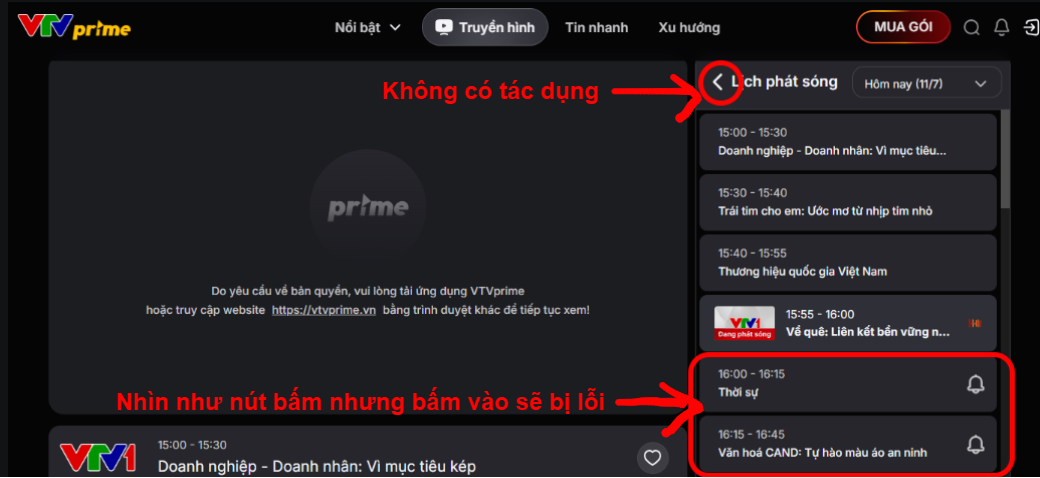
\includegraphics[width=0.6\textwidth]{./vtvprime-product-research-imgs/image23.png}
  \end{center}
\end{itemize}

\subsubsection{Nhược điểm 11: Nút hamburger và nút đóng sidebar trên tablet đặt sai vị trí}

\begin{itemize}
  \item \textbf{Phân tích HCI}: Trên giao diện tablet, nút hamburger (\ensuremath{\ensuremath{\u2630}}) nằm ở sát bên trái navbar --- vị trí này hợp lý. Tuy nhiên, khi bấm vào hamburger thì sidebar mở rộng full màn hình, và nút \ensuremath{\times} (đóng) lại nằm ở \textbf{sát bên phải} màn hình \ensuremath{\rightarrow} khoảng cách di chuyển từ nút hamburger (bên trái) đến nút \ensuremath{\times} (bên phải) rất lớn, buộc người dùng phải di chuyển ngón tay một quãng dài trên tablet --- tăng motor load đáng kể. Theo nguyên tắc \textbf{Reachability \& Motor Load}, các phần tử tương tác thường xuyên nên được đặt ở vị trí dễ chạm tới với nỗ lực vận động tối thiểu.
  \item \textbf{Nguyên tắc liên quan}: Reachability \& Motor Load.
  \item \textbf{Ví dụ cụ thể}:
  \begin{quote}
    Người dùng A đang dùng tablet, muốn truy cập hamburger menu để điều hướng sang trang ``Tin nhanh''. A dùng ngón tay bấm nút hamburger ở góc trên bên trái \ensuremath{\rightarrow} sidebar mở full màn hình. Để đóng sidebar, A phải với tay sang tận góc trên bên phải để bấm nút \ensuremath{\times} \ensuremath{\rightarrow} mất thời gian và bất tiện, đặc biệt với tablet màn hình lớn. Nếu nút \ensuremath{\times} nằm ở vị trí hợp lý hơn (gần nút hamburger hoặc ở mép trái sidebar), thao tác sẽ nhanh hơn rất nhiều.
  \end{quote}
  \begin{center}
    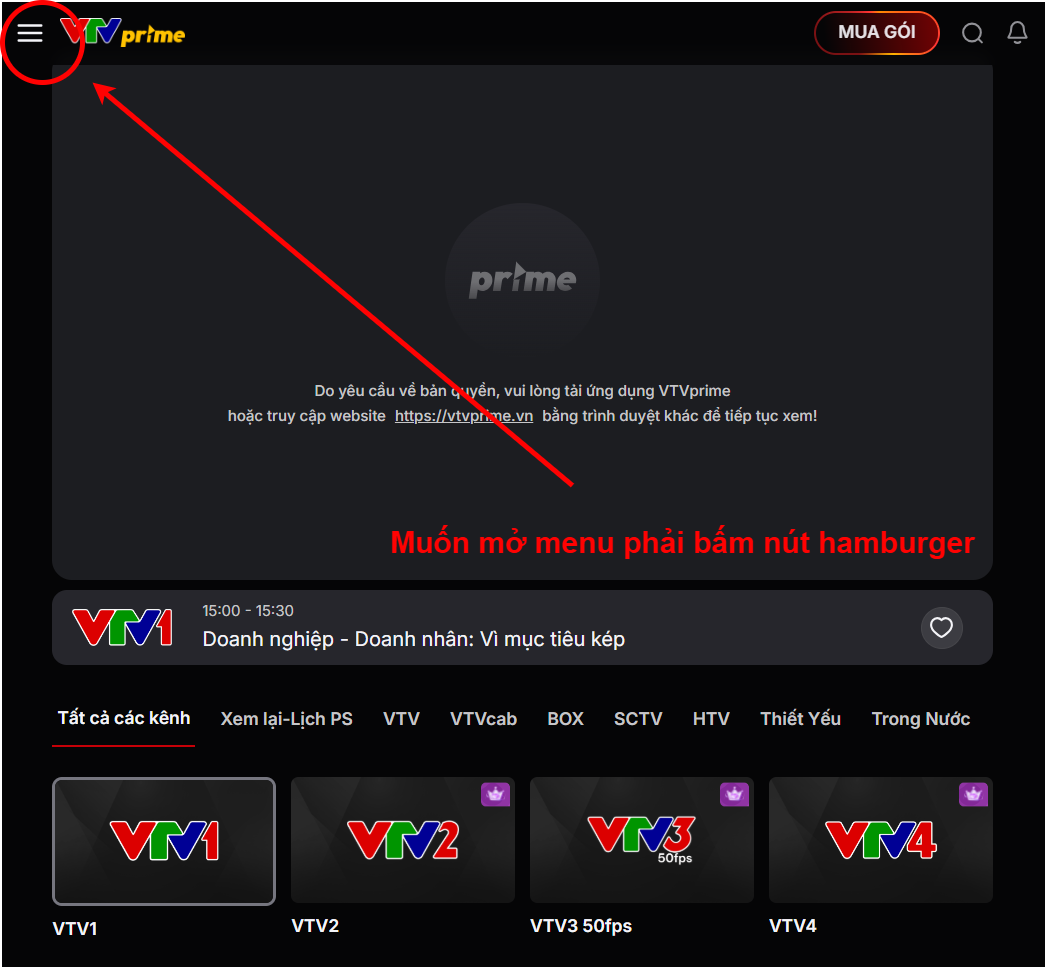
\includegraphics[width=0.6\textwidth]{./vtvprime-product-research-imgs/image24.png}
  \end{center}
  \begin{center}
    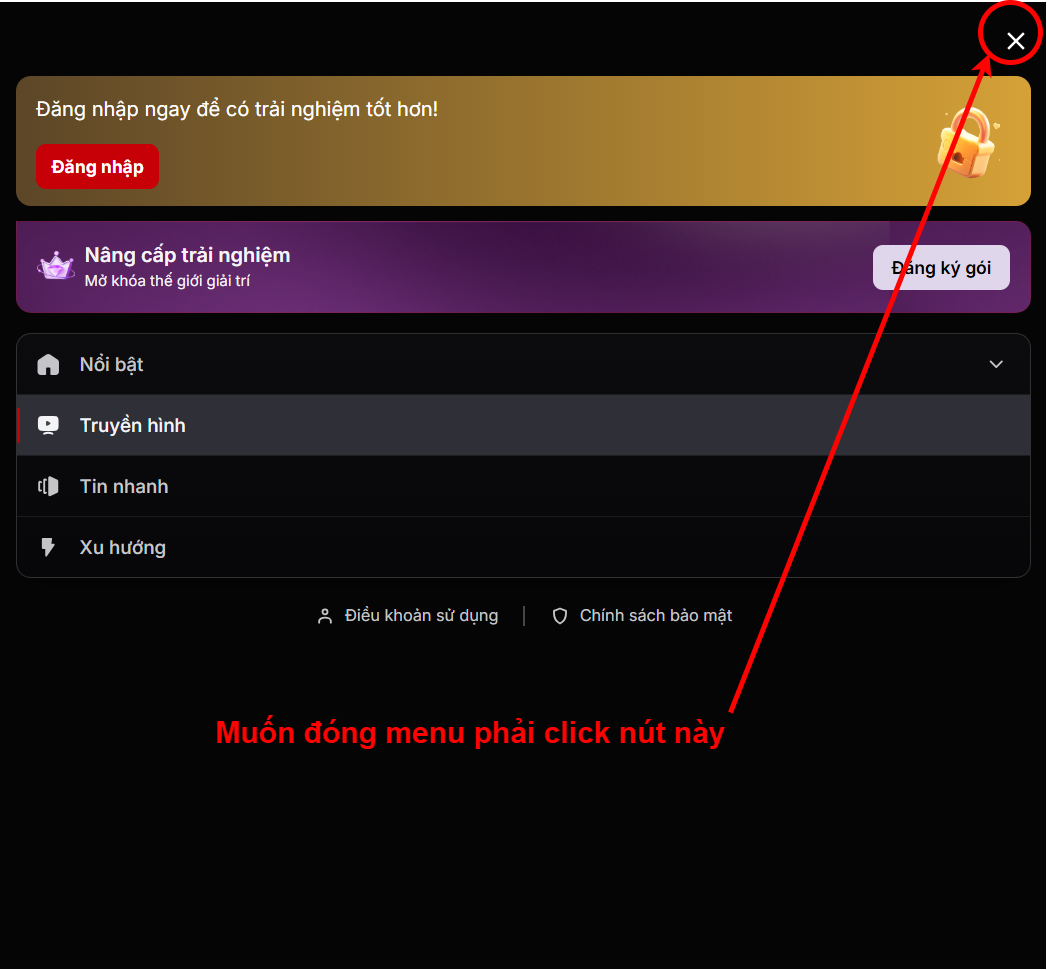
\includegraphics[width=0.6\textwidth]{./vtvprime-product-research-imgs/image25.png}
  \end{center}
  \item \textbf{Đề xuất hướng khắc phục}: (1) Thu nhỏ sidebar lại, không mở rộng full màn hình và làm mờ nội dung ở lớp dưới sidebar, có thể bấm ra ngoài để đóng. (2) Đặt nút \ensuremath{\times} ở sát bên trái sidebar (gần vị trí nút hamburger) thay vì bên phải để giảm khoảng cách di chuyển.
\end{itemize}



% --- 2.5 Các kiểu người dùng & bối cảnh phát sinh khó khăn ---
% Phân tích từ các vấn đề HCI đã tìm ra để xác định người dùng gặp khó khăn
\subsection{Các kiểu người dùng \& bối cảnh phát sinh khó khăn}

Dựa trên phân tích ưu/nhược điểm giao diện ở phần trên, chúng ta có thể xác định những nhóm người dùng nào sẽ gặp khó khăn với từng vấn đề cụ thể. Phân tích này liên kết chặt chẽ với 4 nhóm độ tuổi và 5 phân khúc hành vi đã xác định ở phần trước.

\subsubsection{Vấn đề thiếu thông tin trên thumbnail}

Nhiều carousel trên VTVPrime không hiển thị tên nội dung hoặc mô tả ngắn bên dưới thumbnail, chỉ có thời lượng. Vấn đề này ảnh hưởng đặc biệt đến:

\textbf{Người xem theo dòng sự kiện (Phân khúc 3):} Nhóm này chỉ truy cập khi có sự kiện lớn như World Cup hoặc ASIAD, không thường xuyên sử dụng nền tảng. Khi không thấy tên nội dung trên thumbnail, họ không thể nhận diện nhanh và cảm thấy giao diện khó dùng --- dễ chuyển sang nền tảng khác.

\textbf{Nhóm trung niên (45--54 tuổi):} Nhóm này tiếp cận công nghệ thận trọng và cần cấu trúc rõ ràng. Khi thumbnail thiếu thông tin, họ mất thời gian click vào từng video để hiểu nội dung, làm giảm trải nghiệm sử dụng.

\textbf{Người xem chuyên sâu (Phân khúc 4):} Nhóm này muốn tìm hiểu tường tận chiến thuật và thống kê. Khi thumbnail không hiển thị thông tin chi tiết, họ không thể nhanh chóng xác định nội dung phù hợp với nhu cầu phân tích của mình.

\subsubsection{Vấn đề mũi tên carousel quá nhỏ và đặt sai vị trí}

Mũi tên carousel nhỏ, nằm bên trong carousel trên nền tối, không tận dụng screen edge effect. Vấn đề này ảnh hưởng đặc biệt đến:

\textbf{Nhóm Gen Z (18--24 tuổi):} Đây là thế hệ bản địa số, ưu tiên tốc độ và thao tác nhanh. Mũi tên nhỏ và đặt sai vị trí làm giảm efficiency --- họ phải thao tác chính xác vào vùng nhỏ thay vì có gesture tự nhiên, gây khó hiểu.

\textbf{Người xem đa thiết bị (Phân khúc 5):} Nhóm này thường xuyên chuyển đổi giữa các thiết bị, đặc biệt là thiết bị di động. Mũi tên quá nhỏ để chạm chính xác bằng ngón tay trên màn hình di động, làm giảm trải nghiệm liền mạch khi xem trên nhiều thiết bị.

\textbf{Nhóm người lớn tuổi (55+ tuổi):} Khi thị lực và khả năng vận động giảm, nhóm này gặp khó khăn với các mục tiêu nhỏ trên màn hình. Mũi tên carousel quá nhỏ và trên nền tối khiến họ khó thao tác.

\subsubsection{Vấn đề thiếu feedback cho infinite scroll}

Khi cuộn đến cuối trang, không có thông báo ``đã hết nội dung''. Vấn đề này ảnh hưởng đặc biệt đến:

\textbf{Nhóm Gen Z (18--24 tuổi):} Họ ưu tiên phản hồi tức thì (immediate feedback). Khi không có thông báo, họ không biết trạng thái hệ thống, gây bối rối và giảm trải nghiệm sử dụng.

\textbf{Nhóm lao động trẻ (25--44 tuổi):} Nhóm này có lịch trình bận rộn và đề cao hiệu suất. Khi phải chờ đợi vô ích để ``đoán'' trạng thái hệ thống, họ mất thời gian quý báu và dễ bỏ cuộc.

\textbf{Người xem theo dòng sự kiện (Phân khúc 3):} Nhóm này chưa quen với giao diện. Khi không có feedback, họ có thể nghĩ ứng dụng bị lỗi và thoát ra, làm mất cơ hội giữ chân nhóm này sau sự kiện.

\subsubsection{Vấn đề nút ``Xem tất cả'' không nhất quán}

Một số carousel có nút ``Xem tất cả'', số khác không --- phá vỡ internal consistency. Vấn đề này ảnh hưởng đặc biệt đến:

\textbf{Nhóm trung niên (45--54 tuổi):} Nhóm này ưu tiên cấu trúc rõ ràng và nhất quán. Khi pattern không đồng nhất, họ mất thời gian thích nghi và cảm thấy giao diện khó hiểu.

\textbf{Người xem chuyên sâu (Phân khúc 4):} Nhóm này muốn xem nhanh toàn bộ nội dung để phân tích. Khi nút ``Xem tất cả'' không tồn tại, họ phải lướt thủ công qua toàn bộ carousel --- tốn thời gian và dễ bỏ cuộc nếu carousel quá dài.

\textbf{Nhóm lao động trẻ (25--44 tuổi):} Nhóm này đề cao các patterns quen thuộc để tối ưu hóa thời gian. Khi pattern bị phá vỡ, họ mất thời gian tìm kiếm cách xem toàn bộ nội dung, làm giảm hiệu suất.

\subsubsection{Vấn đề thiếu alt text ảnh}

Nhiều ảnh bị để trống alt text hoặc có alt text vô dụng. Vấn đề này ảnh hưởng đặc biệt đến:

\textbf{Nhóm người lớn tuổi (55+ tuổi):} Khi thị lực giảm, nhóm này phụ thuộc vào screen reader để nhận diện nội dung. Khi alt text bị bỏ trống, họ không thể biết nội dung của thumbnail --- rất bất tiện.

\subsubsection{Vấn đề định dạng card phim bộ không nhất quán}

Cùng là phim bộ nhưng có hai định dạng card khác nhau (định dạng ngang với các lớp chồng lên nhau và định dạng dọc). Vấn đề này ảnh hưởng đặc biệt đến:

\textbf{Nhóm lao động trẻ (25--44 tuổi):} Nhóm này đề cao các patterns quen thuộc. Khi pattern bị phá vỡ, họ phải dừng lại nhận diện lại format, mất thời gian thích nghi và giảm hiệu suất.

\textbf{Nhóm trung niên (45--54 tuổi):} Nhóm này cần cấu trúc rõ ràng và nhất quán. Khi thấy hai định dạng khác nhau cho cùng một loại nội dung, họ cảm thấy giao diện không nhất quán và khó hiểu.

\textbf{Người xem theo dòng sự kiện (Phân khúc 3):} Nhóm này chưa hình thành mental model rõ ràng. Khi định dạng không nhất quán, họ bỡ ngỡ và khó điều hướng, làm giảm trải nghiệm sử dụng.

\subsubsection{Vấn đề lịch phát sóng không phân biệt trạng thái}

Tất cả mục trong lịch phát sóng đều có dạng giống nút bấm, không phân biệt giữa đã phát, đang phát, chưa phát. Vấn đề này ảnh hưởng đặc biệt đến:

\textbf{Người xem theo dòng sự kiện (Phân khúc 3):} Nhóm này chưa quen với quy tắc của lịch phát sóng. Khi thấy tất cả mục đều có dạng nút bấm, họ click vào bất kỳ mục nào và dễ gặp lỗi, làm giảm trải nghiệm sử dụng.

\textbf{Nhóm người lớn tuổi (55+ tuổi):} Nhóm này cần chỉ dẫn cụ thể và rõ ràng. Khi giao diện không phân biệt trạng thái, họ dễ nhầm lẫn và gặp lỗi, tăng cognitive load.

\subsubsection{Vấn đề nút hamburger và nút đóng sidebar trên tablet}

Nút hamburger ở góc trái, nút đóng ở góc phải --- khoảng cách di chuyển lớn. Vấn đề này ảnh hưởng đặc biệt đến:

\textbf{Người xem đa thiết bị (Phân khúc 5):} Nhóm này thường xuyên chuyển đổi giữa các thiết bị, bao gồm tablet. Khi mở sidebar, họ phải với tay từ góc trái sang góc phải để đóng --- mất thời gian và bất tiện, đặc biệt với tablet màn hình lớn.

\textbf{Nhóm người lớn tuổi (55+ tuổi):} Khi khả năng vận động giảm, khoảng cách di chuyển lớn gây khó khăn trong thao tác, tăng motor load đáng kể.

\textbf{Nhóm lao động trẻ (25--44 tuổi):} Nhóm này đề cao efficiency. Khoảng cách di chuyển lớn làm giảm tốc độ thao tác, không phù hợp với nhu cầu tối ưu hóa thời gian của nhóm này.

\bigskip
% ======================================================
%          3. SẢN PHẨM 2: FPTPLAY
% ======================================================
% Cấu trúc tương tự section 2 (VTVPrime) để dễ so sánh
% Bao gồm: Domain, Đối tượng, Use Cases, Phân tích HCI, Kiểu người dùng
\section{Sản phẩm 2: FPTPlay}

% --- 3.1 Tên sản phẩm & Domain ---
% Bảng thông tin tổng quan về FPTPlay
\subsection{Tên sản phẩm \& Domain}

\begin{center}
\begin{tabularx}{\textwidth}{|l|X|}
\hline
\textbf{Thông tin} & \textbf{Chi tiết} \\
\hline
\textbf{Tên sản phẩm} & FPTPlay \\
\hline
\textbf{Domain} & \textbf{Nền tảng OTT (Over-The-Top) --- Truyền hình, phim ảnh \& thể thao trực tuyến.} \\
\hline
\textbf{Nền tảng} & Web (\url{https://fptplay.vn/}), Mobile (iOS/Android) \\
\hline
\textbf{Nhà phát hành} & FPT Telecom \\
\hline
\end{tabularx}
\end{center}

\medskip\noindent\textbf{Phân tích Domain theo 3 khía cạnh:}

\bigskip
\begin{center}
\begin{tabularx}{\textwidth}{|l|X|}
\hline
\textbf{Khía cạnh} & \textbf{Giải thích} \\
\hline
\textbf{\ding{172} Sản phẩm làm về cái gì?} & FPTPlay là ứng dụng OTT do FPT Telecom phát hành, cung cấp nội dung: tường thuật thể thao trực tiếp, kênh truyền hình trực tuyến, phim và chương trình giải trí theo yêu cầu. FPTPlay tiếp sóng World Cup 2026 từ VTV, phát tất cả 104 trận. Ngoài ra còn có truyền hình trực tuyến, phim, chương trình TV và tin tức. Ứng dụng có tích hợp AI để phân tích nội dung thể thao. \\
\hline
\textbf{\ding{173} Dùng trong hoàn cảnh nào?} & Tương tự VTVPrime: người dùng thức khuya xem trực tiếp thể thao (World Cup 2026, các giải đấu quốc tế) do chênh lệch múi giờ. Ban ngày xem lại highlight, tin tức thể thao. Lúc rảnh rỗi xem phim hoặc chương trình giải trí. Thiết bị dùng được: TV thông minh, laptop, máy tính bảng, điện thoại. \\
\hline
\textbf{\ding{174} Quy tắc trong lĩnh vực đó?} & Giống với VTVPrime --- cùng domain OTT thể thao nên có chung 5 yêu cầu: (1) Trận đấu đang diễn ra phải mở được ngay; (2) Nút điều khiển tự ẩn khi xem; (3) Tỉ số, thời gian, tên đội luôn hiển thị; (4) Lịch thi đấu rõ ràng (ngày, giờ, đội); (5) Phân biệt rõ trạng thái Live / Sắp diễn ra / Đã kết thúc. \\
\hline
\end{tabularx}
\end{center}

% --- 3.2 Đối tượng người dùng ---
% Phân khúc người dùng FPTPlay
\subsection{Đối tượng người dùng}

\begin{center}
\begin{tabularx}{\textwidth}{|l|X|}
\hline
\textbf{Nhóm} & \textbf{Mô tả} \\
\hline
\textbf{Người yêu thích thể thao} & Khán giả trung thành, thường xuyên theo dõi các giải đấu độc quyền trên FPTPlay như UEFA Champions League, V-League. Họ quan tâm sâu sắc đến chất lượng đường truyền trực tiếp ổn định, độ phân giải cao (4K/FullHD) và tốc độ cập nhật kết quả. \\
\hline
\textbf{Khán giả phổ thông} & Nhóm người dùng gia đình hoặc khán giả phong trào, chỉ truy cập vào các dịp sự kiện lớn như World Cup 2026 hay ASIAD 2026. Họ coi trọng sự đơn giản, dễ tìm kiếm kênh tiếp sóng và các gói cước gia đình giá rẻ. \\
\hline
\end{tabularx}
\end{center}

\medskip\noindent\textit{Nhận xét:} [Tương tự VTVPrime --- đa dạng đối tượng, độ tuổi, kinh nghiệm sử dụng]

% --- 3.3 Core Use Cases ---
% UC1: Xem live | UC2: Lựa chọn môn thể thao | UC3: Thanh toán gói cước
\subsection{Core Use Cases}

% ---- UC1 ----
\subsubsection{UC1: Xem trực tiếp một trận đấu}

\begin{center}
\begin{tabularx}{\textwidth}{|l|X|}
\hline
\textbf{Khía cạnh} & \textbf{Mô tả} \\
\hline
\textbf{Ở đâu?} & Tại nhà hoặc bất cứ đâu có Internet \\
\hline
\textbf{Khi nào?} & Trước hoặc ngay khi trận đấu bắt đầu \\
\hline
\textbf{Tư thế người dùng} & Ngồi/nằm trên ghế, sofa --- xem trong thời gian dài \\
\hline
\textbf{Thiết bị} & Laptop, điện thoại, máy tính bảng \\
\hline
\end{tabularx}
\end{center}

\medskip\noindent\textbf{Các bước tương tác:}
\begin{enumerate}[leftmargin=2em]
  \item Truy cập FPTPlay $\rightarrow$ đăng nhập (nếu cần).
  \item Banner trận đấu trực tiếp hiển thị $\rightarrow$ chọn ``Xem ngay''.
  \item Sử dụng điều khiển: dừng, âm lượng, phóng to, chất lượng.
\end{enumerate}

\medskip\noindent\textit{Ưu điểm cụ thể (dựa trên HCI):} Hệ thống tự động tối ưu độ phân giải dựa trên tốc độ mạng thực tế (Visibility of System Status), giúp trận đấu không bị ngắt quãng, giảm thiểu sự thất vọng của người dùng khi luồng stream bị nghẽn đột ngột.

\medskip\noindent\textit{Nhược điểm cụ thể (dựa trên HCI):} Khung chat trực tuyến (Live Chat) mặc định hiển thị che khuất một phần góc phải màn hình ở chế độ xem dọc trên điện thoại. Nút ``X'' tắt khung chat quá nhỏ, vi phạm định luật Fitts, khiến người dùng dễ bấm nhầm vào nội dung chat.

% ---- UC2 ----
\subsubsection{UC2: Lựa chọn môn thể thao để xem}

\begin{center}
\begin{tabularx}{\textwidth}{|l|X|}
\hline
\textbf{Khía cạnh} & \textbf{Mô tả} \\
\hline
\textbf{Ở đâu?} & Bất cứ đâu có Internet \\
\hline
\textbf{Khi nào?} & Bất cứ khi nào muốn tìm nội dung thể thao \\
\hline
\textbf{Tư thế người dùng} & Ngồi/nằm --- thao tác duyệt tìm, thời gian ngắn \\
\hline
\textbf{Thiết bị} & Laptop, điện thoại \\
\hline
\end{tabularx}
\end{center}

\medskip\noindent\textbf{Các bước tương tác:}
\begin{enumerate}[leftmargin=2em]
  \item Truy cập FPTPlay.
  \item Trên thanh công cụ $\rightarrow$ ấn ``Xem thêm'' (mũi tên bên phải).
  \item Chọn môn thể thao ưa thích.
  \item Duyệt danh sách trận đấu $\rightarrow$ chọn xem.
\end{enumerate}

\medskip\noindent\textit{Ưu điểm cụ thể (dựa trên HCI):} Các danh mục môn thể thao được minh họa bằng các biểu tượng đặc trưng (Recognition over Recall) như quả bóng đá, quả bóng rổ, giúp người dùng nhận diện thể loại mong muốn ngay lập tức mà không cần đọc chữ.

\medskip\noindent\textit{Nhược điểm cụ thể (dựa trên HCI):} Danh sách môn thể thao khi mở rộng xếp theo dạng thanh cuộn ngang vô tận trên mobile, gây áp lực lên cơ tay (Motor Load) và khiến người dùng khó định vị được các môn nằm ở phía cuối danh sách.

% ---- UC3 ----
\subsubsection{UC3: Lựa chọn và thanh toán gói cước}

\begin{center}
\begin{tabularx}{\textwidth}{|l|X|}
\hline
\textbf{Khía cạnh} & \textbf{Mô tả} \\
\hline
\textbf{Ở đâu?} & Bất cứ đâu có Internet \\
\hline
\textbf{Khi nào?} & Khi cần đăng ký/gia hạn gói thể thao \\
\hline
\textbf{Tư thế người dùng} & Đa dạng --- thao tác ngắn \\
\hline
\textbf{Thiết bị} & Điện thoại (chủ yếu) hoặc laptop \\
\hline
\end{tabularx}
\end{center}

\medskip\noindent\textbf{Các bước tương tác:}
\begin{enumerate}[leftmargin=2em]
  \item Truy cập FPTPlay $\rightarrow$ chọn ``Mua gói'' trên thanh công cụ.
  \item Xem danh sách gói cước $\rightarrow$ chọn gói phù hợp.
  \item Chuyển đến trang thanh toán $\rightarrow$ thực hiện thanh toán.
\end{enumerate}

\medskip\noindent\textit{Ưu điểm cụ thể (dựa trên HCI):} Tích hợp các cổng thanh toán điện tử phổ biến (MoMo, VNPAY) qua mã QR Code giúp rút ngắn hành trình nhập liệu, tăng tốc độ xử lý tác vụ (Efficiency of Use).

\medskip\noindent\textit{Nhược điểm cụ thể (dựa trên HCI):} Giao diện thanh toán thiếu bước tóm tắt đơn hàng rõ ràng trước khi bấm nút xác nhận thanh toán cuối cùng (Error Prevention), dễ dẫn đến việc người dùng mua nhầm gói cước dài hạn mà không hề hay biết.

% --- 3.4 Phân tích ưu điểm dựa trên HCI ---
% 7 nguyên tắc HCI: Recognition, Learnability, Consistency, Capabilities,
% Visibility, Affordances, Mental Model
\subsection{Phân tích ưu điểm dựa trên HCI}

\subsubsection{Recognition \& Recall}
\textbf{Hiện trạng:} Hệ thống sử dụng các icon chuẩn quốc tế cho các tab chức năng chính (Trang chủ, Truyền hình, Thể thao, Phim truyện).\\
\textbf{Phân tích HCI:} Nhấn mạnh cơ chế nhận diện hình ảnh thay vì bắt trí nhớ ngắn hạn làm việc. Người dùng chỉ cần lướt mắt qua là biết vị trí phân mục.\\
\textbf{Ví dụ cụ thể:} Icon chiếc cúp vàng đại diện cho giải đấu World Cup 2026 được ghim cố định ở góc trên giao diện, giúp khán giả click vào ngay mà không cần tìm kiếm thủ công.

\subsubsection{Learnability \& Memorability}
\textbf{Hiện trạng:} Giao diện sắp xếp nội dung dạng lưới thẻ (Grid Cards) trượt ngang, phân vùng nội dung từ trên xuống dưới.\\
\textbf{Phân tích HCI:} Tận dụng tính nhất quán bên ngoài (External Consistency) với các tiêu chuẩn công nghiệp như Netflix hay YouTube, giúp người dùng mới thành thạo ngay trong lần sử dụng đầu tiên.\\
\textbf{Ví dụ cụ thể:} Một người lớn tuổi quen xem phim trên Netflix khi chuyển sang FPTPlay vẫn biết cách vuốt ngang để tìm tập phim tiếp theo nhờ cấu trúc layout tương đồng.

\subsubsection{Consistency}
\textbf{Hiện trạng:} Sắc cam thương hiệu được áp dụng đồng bộ cho tất cả các nút hành động chính (CTA) và trạng thái đang được chọn.\\
\textbf{Phân tích HCI:} Thiết lập tính nhất quán nội bộ (Internal Consistency), giảm thiểu tải nhận thức khi điều hướng qua các màn hình khác nhau.\\
\textbf{Ví dụ cụ thể:} Nút ``Mua gói'' ở trang chủ, nút ``Thanh toán'' ở trang giỏ hàng và các nút ``Xác nhận'' đều dùng chung một mã màu cam và font chữ bo góc đồng nhất.

\subsubsection{Capabilities (Fitts's Law)}
\textbf{Hiện trạng:} Banner các trận đấu Live tiêu điểm của World Cup 2026 được thiết kế với kích thước lớn, chiếm trọn 1/3 phía trên màn hình trang chủ.\\
\textbf{Phân tích HCI:} Áp dụng định luật Fitts: Mục tiêu có kích thước càng lớn ($s$ lớn) thì thời gian tiếp cận và click ($t$) càng ngắn, giúp tăng tỷ lệ nhấp chuột.\\
\textbf{Ví dụ cụ thể:} Khi trận đấu giữa Brazil và Pháp đang diễn ra, người dùng vừa mở app lên là có thể dễ dàng chạm ngón tay vào vùng banner khổng lồ để vào xem trực tiếp ngay lập tức.

\subsubsection{Visibility}
\textbf{Hiện trạng:} Các thẻ trận đấu đang phát trực tiếp luôn được gắn nhãn nhấp nháy chữ ``LIVE'' màu đỏ rực ở góc trái.\\
\textbf{Phân tích HCI:} Đảm bảo nguyên lý Visibility of System Status. Trạng thái thời gian thực của hệ thống được phơi bày rõ ràng trực quan.\\
\textbf{Ví dụ cụ thể:} Giữa một danh sách các trận đấu lưu trữ (replay), người dùng phân biệt được ngay trận nào đang đá trực tiếp dựa vào thẻ nhãn màu đỏ nổi bật.

\subsubsection{Affordances}
\textbf{Hiện trạng:} Các thanh trượt tiến trình (Progress Bar) video có các chấm tròn nổi lên tại điểm mốc thời gian.\\
\textbf{Phân tích HCI:} Gợi ý công năng (Affordance) vật lý rõ ràng: chấm tròn sinh ra là để nắm kéo. Người dùng hiểu ngay hành vi cần làm là kéo thả để tua video.\\
\textbf{Ví dụ cụ thể:} Người dùng không cần đọc hướng dẫn vẫn tự biết dùng ngón tay giữ chấm tròn trên thanh timeline để tua nhanh qua phần quảng cáo đầu trận đấu.

\subsubsection{Mental Model}
\textbf{Hiện trạng:} Danh mục ``Truyền hình'' mô phỏng danh sách kênh theo số thứ tự (VTV1, VTV2, VTV3,\dots) chạy dọc kèm lịch phát sóng theo giờ.\\
\textbf{Phân tích HCI:} Thiết kế trùng khớp với mô hình tâm trí (Mental Model) của người dùng về chiếc TV truyền thống, giúp họ không phải thay đổi thói quen cũ.\\
\textbf{Ví dụ cụ thể:} Người dùng thế hệ trước dễ dàng tìm thấy kênh VTV3 để xem đá bóng bằng cách cuộn tìm số 3 đúng như cách họ bấm remote điều khiển TV ở nhà.

% --- 3.5 Phân tích nhược điểm dựa trên HCI ---
% 3 nhược điểm chính: Capabilities, Visibility (che khuất), Nhược điểm khác
\subsection{Phân tích nhược điểm dựa trên HCI}

\subsubsection{Capabilities --- Không tối ưu cho vùng chạm tay (Reachability)}
\textbf{Hiện trạng:} Nút tìm kiếm (kính lúp) và nút lịch sử xem được đặt ở góc trên cùng bên phải của giao diện di động.\\
\textbf{Phân tích HCI:} Vi phạm nguyên tắc Reachability trên thiết bị di động. Với xu hướng màn hình ngày càng lớn, vùng trên cùng là ``vùng chết'' đối với thao tác một tay.\\
\textbf{Ví dụ cụ thể:} Người dùng cầm điện thoại bằng một tay khi đang đứng trên xe buýt rất khó với ngón cái lên góc trên cùng bên phải để gõ tìm trận đấu World Cup, dễ gây rơi máy.\\
\textbf{Đề xuất hướng khắc phục:} Chuyển thanh tìm kiếm xuống thanh điều hướng dưới cùng (Bottom Navigation Bar) để tối ưu hóa tầm với của ngón tay cái.

\subsubsection{Visibility --- Nội dung quan trọng bị che khuất}
\textbf{Hiện trạng:} Khi xem video ở chế độ màn hình ngang trên điện thoại, các thông báo đẩy (Pop-up thông báo, quảng cáo gói cước) xuất hiện tràn ra giữa màn hình, che khuất bảng tỉ số trận đấu.\\
\textbf{Phân tích HCI:} Vi phạm nghiêm trọng sự tường minh về trạng thái (Visibility). Hệ thống ưu tiên hiển thị quảng cáo hơn nội dung cốt lõi mà người dùng đang theo dõi.\\
\textbf{Ví dụ cụ thể:} Đúng lúc có tình huống nguy hiểm trong vòng cấm, một pop-up quảng cáo ``Gia hạn gói VIP'' hiện lên che mất góc trái màn hình --- nơi hiển thị thời gian trận đấu, gây ức chế cực độ.\\
\textbf{Đề xuất hướng khắc phục:} Định dạng lại thông báo đẩy thành các dòng text nhỏ chạy dưới đáy màn hình hoặc chỉ xuất hiện ở khu vực không có dữ liệu trận đấu.

\subsubsection{Cognitive Load --- Ma trận gói cước gây quá tải nhận thức}
\textbf{Hiện trạng:} Trang thông tin mua gói hiển thị một loạt các gói cước như gói iZi, gói Sport, gói VIP xếp chồng chéo với hàng tá dòng mô tả tính năng chữ nhỏ.\\
\textbf{Phân tích HCI:} Ép buộc người dùng phải sử dụng trí nhớ ngắn hạn (Recall) để so sánh quyền lợi giữa các gói thay vì nhìn thấy trực quan (Recognition), làm chậm quá trình ra quyết định.\\
\textbf{Ví dụ cụ thể:} Người dùng muốn biết gói Sport có xem được phim châu Á như gói VIP không, họ phải click vào từng gói, đọc kỹ rồi tự ghi nhớ và so sánh trong đầu.\\
\textbf{Đề xuất hướng khắc phục:} Xây dựng một bảng ma trận so sánh (Comparison Matrix) với các dấu tích xanh trực quan liệt kê rõ tính năng của từng gói cước cạnh nhau trên một màn hình duy nhất.

% --- 3.6 Các kiểu người dùng & bối cảnh phát sinh khó khăn ---
% Tương tự 2.6 nhưng áp dụng cho FPTPlay
% 6 tình huống: Mới/Quen, Mobile/Desktop, Internet chậm,
% Không rành công nghệ, Ánh sáng mạnh, So sánh gói cước
\subsection{Các kiểu người dùng \& bối cảnh phát sinh khó khăn}

\textit{Yêu cầu:} Xem xét các kiểu người dùng khác nhau và các bối cảnh có thể gây khó khăn/cản trở với giao diện hiện tại.

\subsubsection{3.6.1~Người dùng mới (First-time user) vs Người dùng quen thuộc (Power user)}

\begin{center}
\small
\begin{tabularx}{\textwidth}{|l|X|X|}
\hline
\textbf{Khía cạnh} & \textbf{Người dùng mới} & \textbf{Người dùng quen thuộc} \\
\hline
\textbf{Đặc điểm} & Chưa dùng FPTPlay hoặc các nền tảng OTT trước đây & Đã dùng lâu, biết rõ cấu trúc và tính năng \\
\hline
\textbf{Khó khăn dự kiến} & [Mô tả --- ví dụ: không biết phải ấn ``Xem thêm'' để duyệt môn thể thao] & [Mô tả --- ví dụ: phải qua nhiều bước để vào đúng môn thể thao yêu thích] \\
\hline
\textbf{Bối cảnh cụ thể} & [Tình huống thực tế] & [Tình huống thực tế] \\
\hline
\textbf{Phân tích HCI} & [Learnability, Mental model --- người mới có hiểu ngay cách duyệt không?] & [Efficiency --- số bước thao tác có tối thiểu chưa?] \\
\hline
\end{tabularx}
\end{center}

\subsubsection{3.6.2~Người dùng xem trên thiết bị di động (Mobile) vs Desktop}

\begin{center}
\small
\begin{tabularx}{\textwidth}{|l|X|X|}
\hline
\textbf{Khía cạnh} & \textbf{Mobile} & \textbf{Desktop} \\
\hline
\textbf{Bối cảnh} & Xem khi đi lại, nằm trên giường, trong giờ nghỉ & Xem tại bàn, phòng khách với màn hình lớn \\
\hline
\textbf{Khó khăn dự kiến} & [Mô tả --- ví dụ: phần ``Xem thêm'' ở góc trên cùng, khó với tay khi dùng một tay] & [Mô tả --- ví dụ: các môn thể thao trải dài, phải scroll nhiều] \\
\hline
\textbf{Phân tích HCI} & [Reachability --- nút ở xa tầm với ngón tay cái. Fitts's Law] & [Fitts's Law --- distance lớn, phải di chuyển chuột nhiều] \\
\hline
\end{tabularx}
\end{center}

\subsubsection{3.6.3~Người dùng ở khu vực có kết nối Internet chậm / không ổn định}
\begin{itemize}[leftmargin=2em]
  \item \textbf{Bối cảnh:} Vùng nông thôn, khi di chuyển (xe lửa, xe khách).
  \item \textbf{Khó khăn dự kiến:} [Mô tả --- ví dụ: danh sách gói cước không load kịp, ảnh poster bị vỡ]
  \item \textbf{Phân tích HCI:} [Feedback --- không có indicator nào cho biết đang loading. Error prevention --- dễ bấm nhầm gói cước do giao diện nhảy]
  \item \textbf{Bối cảnh cụ thể:} [Tình huống thực tế]
\end{itemize}

\subsubsection{3.6.4~Người dùng không rành về công nghệ / thanh toán trực tuyến}
\begin{itemize}[leftmargin=2em]
  \item \textbf{Bối cảnh:} Người lớn tuổi, người ít sử dụng Internet, người lo ngại về bảo mật thanh toán.
  \item \textbf{Khó khăn dự kiến:} [Mô tả --- ví dụ: quy trình thanh toán nhiều bước không rõ ràng, sợ bấm nhầm, thiếu hướng dẫn]
  \item \textbf{Phân tích HCI:} [Mental model --- người dùng không có mental model về thanh toán online $\rightarrow$ lo lắng. Error prevention --- thiếu bước xác nhận trước khi thanh toán]
  \item \textbf{Bối cảnh cụ thể:} [Tình huống thực tế]
\end{itemize}

\subsubsection{3.6.5~Người dùng sử dụng trong môi trường ánh sáng mạnh (ngoài trời)}
\begin{itemize}[leftmargin=2em]
  \item \textbf{Bối cảnh:} Xem thông tin thể thao ngoài trời, quán cà phê ngoài trời.
  \item \textbf{Khó khăn dự kiến:} [Mô tả --- ví dụ: chữ trên banner bị chói, khó đọc tên trận đấu]
  \item \textbf{Phân tích HCI:} [Visibility --- thông tin mất khả năng hiển thị. Contrast không đủ cao]
  \item \textbf{Bối cảnh cụ thể:} [Tình huống thực tế]
\end{itemize}

\subsubsection{3.6.6~Người dùng muốn so sánh gói cước nhanh}
\begin{itemize}[leftmargin=2em]
  \item \textbf{Bối cảnh:} Trước khi quyết định mua gói thể thao, người dùng muốn so sánh các gói.
  \item \textbf{Khó khăn dự kiến:} [Mô tả --- ví dụ: phải click vào từng gói để xem chi tiết, không có bảng so sánh cạnh nhau]
  \item \textbf{Phân tích HCI:} [Recognition --- không thể nhìn thấy tất cả thông tin cùng lúc, phải dùng recall để nhớ gói trước khi xem gói sau. Efficiency giảm]
  \item \textbf{Bối cảnh cụ thể:} [Tình huống thực tế]
\end{itemize}

\bigskip

% ======================================================
%          4. TỔNG HỢP & NHẬN XÉT
% ======================================================
% Mục cuối cùng: so sánh và tổng kết 2 sản phẩm
\section{Tổng hợp \& Nhận xét}

% --- 4.1 So sánh nhanh ---
% Bảng đối chiếu 8 tiêu chí HCI giữa VTVPrime và FPTPlay
\subsection{So sánh nhanh giữa hai sản phẩm}

\begin{center}
\small
\begin{tabularx}{\textwidth}{|l|X|X|}
\hline
\textbf{Tiêu chí HCI} & \textbf{VTVPrime} & \textbf{FPTPlay} \\
\hline
Recognition \& Recall & [Nhận xét] & [Nhận xét] \\
\hline
Learnability & [Nhận xét] & [Nhận xét] \\
\hline
Consistency & [Nhận xét] & [Nhận xét] \\
\hline
Capabilities (Fitts) & [Nhận xét] & [Nhận xét] \\
\hline
Error Prevention & [Nhận xét] & [Nhận xét] \\
\hline
Feedback & [Nhận xét] & [Nhận xét] \\
\hline
Reachability & [Nhận xét] & [Nhận xét] \\
\hline
Inclusive Design & [Nhận xét] & [Nhận xét] \\
\hline
\end{tabularx}
\end{center}

% --- 4.2 Kết luận ---
% Tổng kết điểm mạnh/yếu, gợi mở cho phần Potential Solutions
\subsection{Kết luận}

[Tổng kết ngắn gọn: những điểm mạnh/yếu chính của cả 2 sản phẩm, gợi mở cho phần Potential Solutions]

\bigskip

% ======================================================
%          TÀI LIỆU THAM KHẢO
% ======================================================
% Liệt kê các nguồn đã sử dụng trong bài nghiên cứu
\section{Tài liệu tham khảo}

\begin{enumerate}
    \item DataReportal. (2026). Digital 2026: Vietnam. https://datareportal.com/reports/digital-2026-vietnam \label{ref:datareportal}
    \item VietnamFinance. (2025). Báo cáo ``Nhu cầu Giải trí số Việt Nam 2024--2025''. https://vietnamfinance.vn/bao-cao-nhu-cau-giai-tri-so-viet-nam-2024-2025-d128168.html \label{ref:vietnamfinance}
    \item Adwave. (2025). Sports Streaming Statistics: Where Fans Are Watching. https://adwave.com/resources/sports-fans-streaming-statistics \label{ref:adwave}
    \item Antenna. (2025). Sports Streaming Demographics. https://www.antenna.live/insights/sports-streaming-demographics \label{ref:antenna}
    \item InterDigital \& Parks Associates. (2025). Streaming Live Sports: Where Opportunity Meets Complexity. https://www.interdigital.com/white\_papers/streaming-live-sports-where-opportunity-meets-complexity \label{ref:interdigital}
    \item Performance Research. (2025). Nine in 10 sports fans are streaming sports. https://www.sportsbusinessjournal.com/Articles/2025/07/03/study-nine-in-10-sports-fans-are-streaming-sports/ \label{ref:performanceresearch}
    \item Kantar. (2026). Understanding modern sports fans: Why fanatics lead the game. https://www.kantar.com/inspiration/research-services/understanding-modern-sports-fans-pf \label{ref:kantar}
    \item Applicaster. (2026). 2026 Quick Guide: How to Engage Every Type of Digital Sports Fan. https://www.applicaster.com/resources/engaged-every-sports-fan \label{ref:applicaster}
    \item N3XT Sports. (2022). The importance of fan segmentation: how to turn data into engagement. https://www.n3xtsports.com/the-importance-of-fan-segmentation/ \label{ref:n3xtsports}
\end{enumerate}

% ======================================================
%          PHỤ LỤC
% ======================================================
\appendix
\section{Các nguyên tắc HCI}

\subsection{Recognition \& Recall (Nhận diện \& Nhớ lại)}

\textbf{Recognition} là khả năng người dùng nhận diện được thông tin hoặc chức năng cần thiết khi quan sát giao diện --- thông tin được hiển thị sẵn, người dùng chỉ cần nhìn và xác nhận. \textbf{Recall} là khả năng nhớ lại thông tin từ trí nhớ dài hạn mà không có manh mối trực quan hỗ trợ. Trong thiết kế giao diện, recognition được coi là hiệu quả hơn recall vì giảm thiểu nỗ lực nhận thức của người dùng.

\subsection{Learnability (Khả năng học)}

Learnability đo lường thời gian và nỗ lực cần thiết để người dùng mới có thể sử dụng hệ thống đạt hiệu suất cơ bản mà không mắc lỗi. Đây là một trong năm tiêu chí cốt lõi của Usability theo khung đánh giá của Nielsen.

\subsection{Memorability (Khả năng ghi nhớ)}

Memorability là khả năng người dùng có thể tái lập thao tác sử dụng hệ thống sau một khoảng thời gian gián đoạn mà không cần phải học lại từ đầu. Bố cục giao diện tuân theo các khuôn mẫu (pattern) nhất quán và lặp lại sẽ hỗ trợ memorability.

\subsection{Efficiency / Fitts's Law (Hiệu quả)}

Fitts's Law là mô hình toán học mô tả mối quan hệ giữa thời gian di chuyển đến mục tiêu với khoảng cách và kích thước của mục tiêu đó:

\[t = a + b \cdot \log_2\left(\frac{d}{s} + 1\right)\]

Trong đó $d$ là khoảng cách từ vị trí hiện tại đến tâm mục tiêu, $s$ là kích thước (chiều rộng) của mục tiêu, $a$ và $b$ là hằng số phụ thuộc ngữ cảnh. Theo công thức này, mục tiêu càng lớn và càng gần thì thời gian tương tác càng ngắn.

\subsection{Error Prevention (Phòng ngừa lỗi)}

Error Prevention yêu cầu hệ thống được thiết kế để ngăn chặn lỗi trước khi chúng xảy ra, thay vì chỉ cung cấp cơ chế khắc phục sau khi lỗi đã xảy ra. Biện pháp phòng ngừa bao gồm: đặt các hành động nguy hiểm ở vị trí khó vô tình kích hoạt, yêu cầu xác nhận trước khi thực hiện các thao tác không thể hoàn tác, và cung cấp hướng dẫn trực quan để người dùng thực hiện thao tác đúng ngay từ lần đầu.

\subsection{Accessibility / Inclusive Design (Khả năng tiếp cận \& Thiết kế toàn diện)}

Accessibility là nguyên tắc đảm bảo giao diện có thể được sử dụng bởi tất cả đối tượng người dùng, bao gồm cả những người có hạn chế về thị giác, thính giác, vận động hoặc nhận thức. Một ví dụ điển hình về yếu tố giúp cải thiện accessibility là \textbf{contrast ratio} --- tỉ số độ sáng giữa phần tử cần đọc (chữ, icon, hình ảnh) và nền đằng sau nó. Contrast ratio được tính theo công thức W3C dựa trên độ sáng tương đối (relative luminance) của hai lớp màu: lớp foreground (chữ, icon) và lớp background (nền). Thang đo từ 1:1 (foreground và nền trùng màu hoàn toàn, không đọc được) đến 21:1 (đen trắng thuần, tương phản cao nhất). Contrast ratio càng cao thì chữ càng dễ đọc, đặc biệt quan trọng với người dùng khiếm thị nhẹ hoặc người dùng trong điều kiện ánh sáng yếu (ngoài trời nắng, màn hình mờ).

Để đánh giá một giao diện có đạt chuẩn accessibility hay không, các nhà thiết kế dựa vào \textbf{WCAG} (Web Content Accessibility Guidelines) --- bộ tiêu chuẩn quốc tế do W3C phát hành, quy định các yêu cầu tối thiểu mà giao diện web phải đáp ứng để người dùng khuyết tật có thể truy cập và sử dụng được. Trong đó, yêu cầu về contrast ratio là một trong những tiêu chí quan trọng nhất: $\geq$ 4.5:1 cho văn bản thông thường và $\geq$ 3:1 cho văn bản lớn ($\geq$ 18px hoặc $\geq$ 14px bold). Ngoài ra, WCAG còn yêu cầu tất cả phần tử tương tác phải có tên mô tả cho trình đọc màn hình (screen reader), và cấu trúc heading phải tuân theo thứ tự phân cấp. Khoảng 7--8\% nam giới mắc chứng mù màu (color blindness), vì vậy giao diện không nên dựa duy nhất vào màu sắc để truyền tải thông tin.

\subsection{Attention \& Cognitive Load (Sự chú ý \& Tải nhận thức)}

Hệ thống nhận thức của con người xử lý thông tin thông qua ba cơ chế chú ý chính: \textbf{Selective attention} (lọc và tập trung vào một nguồn thông tin giữa nhiều nguồn), \textbf{Focused attention} (tập trung hoàn toàn vào một đối tượng, loại bỏ mọi yếu tố xung quanh), và \textbf{Divided attention} (phân bổ sự chú ý đồng thời cho nhiều nguồn thông tin). Working memory (bộ nhớ ngắn hạn) có dung lượng hạn chế, chỉ lưu giữ được khoảng 7--10 đơn vị thông tin (chunks) tại một thời điểm. Khi giao diện hiển thị quá nhiều thông tin đồng thời, người dùng rơi vào tình trạng cognitive overload (quá tải nhận thức).

\subsection{Reachability \& Motor Load (Tầm với \& Tải vận động)}

Reachability đề cập đến khả năng người dùng có thể chạm tới các phần tử tương tác trên giao diện với nỗ lực vận động tối thiểu. Motor Load là thước đo nỗ lực vận động (di chuyển tay, ngón tay, con trỏ chuột) cần thiết để thực hiện một thao tác.

\subsection{Mental Model \& Metaphor (Mô hình tinh thần \& Ẩn dụ)}

\textbf{Mental model} là cấu trúc nhận thức bên trong tâm trí người dùng về cách một hệ thống hoạt động, được hình thành dựa trên kinh nghiệm và trải nghiệm tương tác trước đó. Khi giao diện phù hợp với mental model, người dùng có thể sử dụng hiệu quả mà không cần học lại; khi đi ngược lại mental model, người dùng sẽ gặp khó khăn và phải thử sai. \textbf{Metaphor} (ẩn dụ thiết kế) là kỹ thuật vay mượn hình ảnh, biểu tượng hoặc cách tương tác từ các đối tượng quen thuộc trong thế giới vật lý để áp dụng lên các đối tượng trong giao diện số.

\subsection{Consistency (Tính nhất quán)}

Consistency gồm hai loại chính: \textbf{Internal consistency} (Nhất quán nội bộ) --- các phần tử cùng chức năng trong một ứng dụng phải hoạt động và được thể hiện giống nhau ở mọi nơi. \textbf{External consistency} (Nhất quán bên ngoài) --- giao diện nên tuân theo các tiêu chuẩn và khuôn mẫu phổ biến mà người dùng đã quen thuộc từ các ứng dụng khác trong cùng lĩnh vực. Consistency giúp người dùng chỉ cần học cách tương tác một lần và có thể áp dụng kiến thức đó ở mọi nơi.

\subsection{Affordances \& Natural Mapping (Tính gợi ý \& Ánh xạ tự nhiên)}

\textbf{Affordance} (theo Don Norman) là thuộc tính của đối tượng thiết kế gợi ý cho người dùng biết cách sử dụng nó --- nút nổi lên trên bề mặt gợi ý thao tác nhấn, thanh trượt gợi ý thao tác kéo. \textbf{Natural Mapping} là mối quan hệ tự nhiên và trực giác giữa cơ chế điều khiển (control) và kết quả tác động (effect) --- mũi tên bên phải tương ứng với việc di chuyển nội dung sang bên phải, cần lái xe quay trái thì phương tiện rẽ trái.

\subsection{Visibility (Tính hiển thị)}

Visibility yêu cầu giao diện phải thể hiện rõ ràng tất cả các chức năng khả dụng và trạng thái hiện tại của hệ thống. Người dùng cần biết được: hệ thống có thể thực hiện những thao tác gì, thao tác nào đang khả dụng tại thời điểm hiện tại, và hệ thống đang ở giai đoạn nào của quy trình xử lý. Thách thức trong thiết kế là cân bằng giữa visibility và simplicity --- hiển thị đủ thông tin nhưng giữ giao diện đơn giản.

\subsection{Feedback (Phản hồi)}

Feedback là nguyên tắc yêu cầu hệ thống phải cung cấp phản hồi trực quan và rõ ràng sau mỗi hành động của người dùng. Khi người dùng thực hiện một thao tác (nhấn nút, cuộn trang, nhập dữ liệu), hệ thống cần xác nhận rằng thao tác đã được nhận diện và hiển thị kết quả hoặc trạng thái tương ứng. Thiếu feedback dẫn đến tình trạng người dùng không biết hệ thống có đang hoạt động hay không, gây cảm giác bất an và giảm niềm tin vào hệ thống.

